%%%%%%%%%%%%%%%%%%%%%%%%%%%%%%%%%%%%%%%%%%%%%%%%%%%%%%%%%%%%%%%%
%
% Apuntes de la asignatura Modelos Matemáticos I.
% Doble Grado de Informática y Matemáticas.
% Universidad de Granada.
% Curso 2016/17.
% 
% 
% Colaboradores:
% Javier Sáez (@fjsaezm)
% Daniel Pozo (@danipozodg)
% Pedro Bonilla (@pedrobn23)
% Guillermo Galindo (@guillegalor)
% Antonio Coín (@antcc)
% Sofía Almeida (@SofiaAlmeida)
% Jesús Sánchez de Lechina (@jojelupipa)
%
% Agradecimientos:
% Andrés Herrera (@andreshp) y Mario Román (@M42) por
% las plantillas base.
%
% Sitio original:
% https://github.com/libreim/apuntesDGIIM/
%
% Licencia:
% CC BY-NC-SA 4.0 (https://creativecommons.org/licenses/by-nc-sa/4.0/)
%
%%%%%%%%%%%%%%%%%%%%%%%%%%%%%%%%%%%%%%%%%%%%%%%%%%%%%%%%%%%%%%%


%------------------------------------------------------------------------------
%   ACKNOWLEDGMENTS
%------------------------------------------------------------------------------

%%%%%%%%%%%%%%%%%%%%%%%%%%%%%%%%%%%%%%%%%%%%%%%%%%%%%%%%%%%%%%%%%%%%%%%%
% Plantilla básica de Latex en Español.
%
% Autor: Andrés Herrera Poyatos (https://github.com/andreshp) 
%
% Es una plantilla básica para redactar documentos. Utiliza el paquete  fancyhdr para darle un
% estilo moderno pero serio.
%
% La plantilla se encuentra adaptada al español.
%
%%%%%%%%%%%%%%%%%%%%%%%%%%%%%%%%%%%%%%%%%%%%%%%%%%%%%%%%%%%%%%%%%%%%%%%%%

%%%
% Plantilla de Trabajo
% Modificación de una plantilla de Latex de Frits Wenneker para adaptarla 
% al castellano y a las necesidades de escribir informática y matemáticas.
%
% Editada por: Mario Román
%
% License:
% CC BY-NC-SA 3.0 (http://creativecommons.org/licenses/by-nc-sa/3.0/)
%%%

%%%%%%%%%%%%%%%%%%%%%%%%%%%%%%%%%%%%%%%%
% Short Sectioned Assignment
% LaTeX Template
% Version 1.0 (5/5/12)
%
% This template has been downloaded from:
% http://www.LaTeXTemplates.com
%
% Original author:
% Frits Wenneker (http://www.howtotex.com)
%
% License:
% CC BY-NC-SA 3.0 (http://creativecommons.org/licenses/by-nc-sa/3.0/)
%
%%%%%%%%%%%%%%%%%%%%%%%%%%%%%%%%%%%%%%%%%


% Tipo de documento y opciones.
%\documentclass[11pt, a4paper, twoside]{article} % Usar para imprimir
\documentclass[11pt, a4paper]{article}


%---------------------------------------------------------------------------
%   PAQUETES
%---------------------------------------------------------------------------

% Idioma y codificación para Español.
\usepackage[utf8]{inputenc}
\usepackage[spanish, es-tabla, es-lcroman, es-noquoting]{babel}
\selectlanguage{spanish} 
%\usepackage[T1]{fontenc}

% Fuente utilizada.
\usepackage{courier}    % Fuente Courier.
\usepackage{microtype}  % Mejora la letra final de cara al lector.

% Diseño de página.
\usepackage{fancyhdr}   % Utilizado para hacer títulos propios.
\usepackage{titlesec} 	% Utilizado para hacer títulos propios.
\usepackage{lastpage}   % Referencia a la última página.
\usepackage{extramarks} % Marcas extras. Utilizado en pie de página y cabecera.
\usepackage[parfill]{parskip}    % Crea una nueva línea entre párrafos.
\usepackage{geometry}            % Geometría de las páginas.

% Símbolos y matemáticas.
\usepackage{amssymb, amsmath, amsthm, amsfonts, amscd}
\usepackage{upgreek}

\usepackage{mdframed}

% Otros.
\usepackage{enumitem}   % Listas mejoradas.
\usepackage[hidelinks]{hyperref}
\usepackage{pgfplots}
\usepackage{graphicx}            % Gráficos.
\usepackage{float}

% Dibujos Tikz
\usepackage{pgf,tikz}
\usepackage{mathrsfs}
\usetikzlibrary{arrows,calc,intersections,through,backgrounds}

% Fuentes personalizadas
\usepackage[scaled=.85]{newpxtext,newpxmath}
\usepackage[scaled=.85]{FiraSans}
\usepackage[T1]{fontenc}

% Código para ajustar las fuentes matemáticas al estilo del texto
% que le rodea

\DeclareMathVersion{sans}
\SetSymbolFont{operators}{sans}{OT1}{cmbr}{m}{n}
\SetSymbolFont{letters}{sans}{OML}{cmbr}{m}{it}
\SetSymbolFont{symbols}{sans}{OMS}{cmbrs}{m}{n}
\SetMathAlphabet{\mathit}{sans}{OT1}{cmbr}{m}{sl}
\SetMathAlphabet{\mathbf}{sans}{OT1}{cmbr}{bx}{n}
\SetMathAlphabet{\mathtt}{sans}{OT1}{cmtl}{m}{n}
\SetSymbolFont{largesymbols}{sans}{OMX}{iwona}{m}{n}

\DeclareMathVersion{boldsans}
\SetSymbolFont{operators}{boldsans}{OT1}{cmbr}{b}{n}
\SetSymbolFont{letters}{boldsans}{OML}{cmbrm}{b}{it}
\SetSymbolFont{symbols}{boldsans}{OMS}{cmbrs}{b}{n}
\SetMathAlphabet{\mathit}{boldsans}{OT1}{cmbr}{b}{sl}
\SetMathAlphabet{\mathbf}{boldsans}{OT1}{cmbr}{bx}{n}
\SetMathAlphabet{\mathtt}{boldsans}{OT1}{cmtl}{b}{n}
\SetSymbolFont{largesymbols}{boldsans}{OMX}{iwona}{bx}{n}

\newif\IfInSansMode
\let\oldsf\sffamily
\renewcommand*{\sffamily}{\oldsf\mathversion{sans}\InSansModetrue}
\let\oldmd\mdseries
\renewcommand*{\mdseries}{\oldmd\IfInSansMode\mathversion{sans}\fi\relax}
\let\oldbf\bfseries
\renewcommand*{\bfseries}{\oldbf\IfInSansMode\mathversion{boldsans}\else%
   \mathversion{bold}\fi\relax}
\let\oldnorm\normalfont
\renewcommand*{\normalfont}{\oldnorm\InSansModefalse\mathversion{normal}}
\let\oldrm\rmfamily
\renewcommand*{\rmfamily}{\oldrm\InSansModefalse\mathversion{normal}}

% Colores

\definecolor{50}{HTML}{E3F2FD}
\definecolor{300}{HTML}{64B5F6}
\definecolor{500}{HTML}{2196F3}
\definecolor{700}{HTML}{1976D2}
\definecolor{900}{HTML}{0D47A1}

%---------------------------------------------------------------------------
%   OPCIONES PERSONALIZADAS
%---------------------------------------------------------------------------

% Redefinir letra griega épsilon.
\let\epsilon\upvarepsilon

% Formato de texto.
\linespread{1.3}            % Espaciado entre líneas.
\setlength\parindent{0pt}   % No indentar el texto por defecto.
\setlist{leftmargin=.5in}   % Indentación para las listas.

% Estilo de página.
\pagestyle{fancy}
\fancyhf{}
\geometry{left=3cm,right=3cm,top=3cm,bottom=3cm}   % Márgenes y cabecera.

% Estilo de las cabeceras

\titleformat{\section}
  {\Large\bfseries\sffamily}{\thesection}{1em}{}
\titleformat{\subsection}
  {\large\sffamily}{\thesubsection}{1em}{}
\titleformat{\subsubsection}
  {\normalsize\sffamily}{\thesubsubsection}{1em}{}

% Estilo de enlaces
\hypersetup{
  % hidelinks = true,   % Oculta todos los enlaces.
  colorlinks = true,   % Muestra todos los enlaces, sin bordes alrededor.
  linkcolor=black,     % Color de enlaces genéricos
  citecolor={blue!50!black},   % Color de enlaces de referencias
  urlcolor={blue!80!black}     % Color de enlaces de URL
}

% Ruta donde buscar gráficos
\graphicspath{{../Recursos/Plantillas/}, {Recursos/Plantillas/}}

% Redefinir entorno de demostración (reducir espacio superior)
\makeatletter
\renewenvironment{proof}[1][\proofname] {\vspace{-15pt}\par\pushQED{\qed}\normalfont\topsep6\p@\@plus6\p@\relax\trivlist\item[\hskip\labelsep\it#1\@addpunct{.}]\ignorespaces}{\popQED\endtrivlist\@endpefalse}
\makeatother

% Aumentar el tamaño del interlineado
\linespread{1.3}

% Numerar las ecuaciones del entorno {equation} con respecto a las secciones
\numberwithin{equation}{section}


%---------------------------------------------------------------------------
%   COMANDOS PERSONALIZADOS
%---------------------------------------------------------------------------

% Valor absoluto: \abs{}
\providecommand{\abs}[1]{\lvert#1\rvert}    

% Fracción grande: \ddfrac{}{}
\newcommand\ddfrac[2]{\frac{\displaystyle #1}{\displaystyle #2}}

% Texto en negrita en modo matemática: \bm{}
\newcommand{\bm}[1]{\boldsymbol{#1}}

% Línea horizontal.
\newcommand{\horrule}[1]{\rule{\linewidth}{#1}}

% Renombrar la R de los reales
\newcommand{\R}{\mathbb{R}}

% Flechitas de los vectores de tamaño apropiado
\renewcommand{\vec}{\overrightarrow}

% Letra lambda
\newcommand{\la}{\lambda}

% Polinomio característico
\newcommand{\pl}{p(\lambda)}

% Matriz 2x2
\newcommand{\m}[4]{%
  \begin{pmatrix} #1 & #2 \\ #3 & #4\end{pmatrix}
}

% Matriz 3x3
\newcommand{\mm}[9]{%
  \begin{pmatrix} #1 & #2 & #3\\ #4 & #5 & #6\\ #7 & #8 & #9\end{pmatrix}
}

% Determinante 2x2
\newcommand{\detm}[4]{%
  \begin{vmatrix} #1 & #2 \\ #3 & #4\end{vmatrix}
}
% Determinante 3x3
\newcommand{\detmm}[9]{%
  \begin{vmatrix} #1 & #2 & #3\\ #4 & #5 & #6\\ #7 & #8 & #9\end{vmatrix}
}

%---------------------------------------------------------------------------
%   CABECERA Y PIE DE PÁGINA
%---------------------------------------------------------------------------

\renewcommand{\sectionmark}[1]{%
\markboth{#1}{}} 

\renewcommand{\subsectionmark}[1]{%
\markright{#1}{}}

%\addtolength{\headheight}{4ex}
\renewcommand{\headrulewidth}{0pt}

\addtolength{\headwidth}{\marginparsep}
%\addtolength{\headwidth}{\marginparwidth}

\fancypagestyle{section}{%
  \fancyhead{}
  %\addtolength{\headheight}{-10ex}
  %\renewcommand{\headheight}{0pt}%
  %\setlength{\footskip}{-48pt}%
  \fancyfoot[LE,RO]{\Large\sffamily\thepage}
  \renewcommand{\headrulewidth}{0pt}%
  \renewcommand{\footrulewidth}{0pt}%
}

\let\originalsection\section
\RenewDocumentCommand{\section}{som}{%
  \IfBooleanTF{#1}
    {\originalsection*{#3}}
    {\IfNoValueTF{#2}
      {\originalsection{#3}}
      {\originalsection[#2]{#3}}%
    }%
  \thispagestyle{section}%
}

% Texto del pie de página.

\fancyhead[LE,RO]{\sffamily\textsl{\rightmark}}
\cfoot{}                                                 % Centro.
\fancyhead[LO,RE]{\sffamily{\leftmark}}
\fancyfoot[LE,RO]{\Large\sffamily\thepage}


%---------------------------------------------------------------------------
%   ENTORNOS PARA MATEMÁTICAS
%---------------------------------------------------------------------------

% Nuevo estilo para definiciones.
\newtheoremstyle{definition-style} % Nombre del estilo.
{}               % Espacio por encima.
{}               % Espacio por debajo.
{}                   % Fuente del cuerpo.
{}                   % Identación.
{\bf\sffamily}                % Fuente para la cabecera.
{.}                  % Puntuación tras la cabecera.
{.5em}               % Espacio tras la cabecera.
{\thmname{#1}\thmnumber{ #2}\thmnote{ (#3)}}     % Especificación de la cabecera (actual: nombre en negrita).

% Nuevo estilo para notas.
\newtheoremstyle{remark-style} 
{10pt}                
{10pt}                
{}                   
{}                   
{\itshape \sffamily}          
{.}                  
{.5em}               
{}                  

% Nuevo estilo para teoremas y proposiciones.
\newtheoremstyle{theorem-style}
{}                
{}                
{}           
{}                  
{\bfseries \sffamily}             
{.}                
{.5em}           
{\thmname{#1}\thmnumber{ #2}\thmnote{ (#3)}}

% Nuevo estilo para ejemplos.
\newtheoremstyle{example-style}
{10pt}                
{10pt}                
{}                  
{}                   
{\bf \sffamily}              
{}                 
{.5em}               
{\thmname{#1}\thmnumber{ #2.}\thmnote{ #3.}}  

% Nuevo estilo para la demostración
%\renewenvironment{proof}{{\itshape \sffamily Demostración \\}}{\hspace*{\fill}\qed}

\makeatletter
\renewenvironment{proof}[1][\proofname] {\par\pushQED{\qed}\normalfont\topsep6\p@\@plus6\p@\relax\trivlist\item[\hskip\labelsep\itshape\sffamily#1\@addpunct{.}]\ignorespaces}{\popQED\endtrivlist\@endpefalse}
\makeatother

% Configuración general de mdframe, los estilos de los teoremas, etc
\mdfsetup{skipabove=12pt,skipbelow=12pt,innertopmargin=12pt,innerbottommargin=4pt}

% Creamos los 'marcos' de los estilos

\mdfdefinestyle{nth-frame}{
	linewidth=2pt, %
	linecolor= 500, % 
	%linecolor=black,
	topline=false, %
	bottomline=false, %
	rightline=false,%
	leftmargin=0pt, %
	innerleftmargin=1em, % 
	rightmargin=0pt, %
	innerrightmargin=0pt, % % 
	%splittopskip=\topskip, %
	%splitbottomskip=\topskip, %
}% 

\mdfdefinestyle{nprop-frame}{
	linewidth=2pt, %
	linecolor= 300, %
	%linecolor= gray, 
	topline=false, %
	bottomline=false, %
	rightline=false,%
	leftmargin=0pt, %
	innerleftmargin=1em, %
	innerrightmargin=0em, 
	rightmargin=0pt, %
	%splittopskip=\topskip, %
	%splitbottomskip=\topskip, %
}%       

\mdfdefinestyle{ndef-frame}{
	linewidth=2pt, %
	linecolor= 300, % 
	%linecolor= gray!50,
	backgroundcolor= 50,
	%backgroundcolor= gray!5,
	topline=false, %
	bottomline=false, %
	rightline=false,%
	leftmargin=0pt, %
	innerleftmargin=1em, %
	innerrightmargin=1em, 
	rightmargin=0pt, % 
	innertopmargin=1.5em,%
	innerbottommargin=1em, % 
	splittopskip=\topskip, %
	%splitbottomskip=\topskip, %
}%         

\mdfdefinestyle{ejemplo-frame}{
	linewidth=0pt, %
	linecolor= 300, % 
	%backgroundcolor= 50,
	leftline=false, %
	rightline=false, %
	leftmargin=0pt, %
	innerleftmargin=1.5em, %
	innerrightmargin=1.5em, 
	rightmargin=0pt, % 
	innertopmargin=0em,%
	innerbottommargin=0em, % 
	splittopskip=\topskip, %
	%splitbottomskip=\topskip, %
}%    

% Asignamos los marcos a los estilos

\surroundwithmdframed[style=nth-frame]{nth}
\surroundwithmdframed[style=nprop-frame]{nprop}
\surroundwithmdframed[style=nprop-frame]{ncor}
\surroundwithmdframed[style=ndef-frame]{ndef}
\surroundwithmdframed[style=ejemplo-frame]{ejemplo}              

% Teoremas, proposiciones y corolarios.
\theoremstyle{theorem-style}
\newtheorem{nth}{Teorema}[section]
\newtheorem{nprop}{Proposición}[section]
\newtheorem{ncor}{Corolario}[section]
\newtheorem{lema}{Lema}[section]

% Definiciones.
\theoremstyle{definition-style}
\newtheorem{ndef}{Definición}[section]

% Notas.
\theoremstyle{remark-style}
\newtheorem*{nota}{Nota}

% Ejemplos.
\theoremstyle{example-style}
\newtheorem{ejemplo}{Ejemplo}[section]

% Listas ordenadas con números romanos (i), (ii), etc.
\newenvironment{nlist}
{\begin{enumerate}
    \renewcommand\labelenumi{(\emph{\roman{enumi})}}}
  {\end{enumerate}}

% División por casos con llave a la derecha.
\newenvironment{rcases}
  {\left.\begin{aligned}}
  {\end{aligned}\right\rbrace}

%---------------------------------------------------------------------------
%   PÁGINA DE TÍTULO
%---------------------------------------------------------------------------

% Título del documento.
\newcommand{\subject}{Modelos Matemáticos I}

% Autor del documento.
\newcommand{\docauthor}{Doble Grado de Informática y Matemáticas}

% Título
\title{
  \normalfont \normalsize 
  \textsc{Universidad de Granada} \\ [25pt]    % Texto por encima.
  \horrule{0.5pt} \\[0.4cm] % Línea horizontal fina.
  \huge \sffamily\subject\\ % Título.
  \horrule{2pt} \\[0.5cm] % Línea horizontal gruesa.
}

% Autor.
\author{\Large\sffamily{\docauthor}}

% Fecha.
\date{\vspace{-1.5em} \normalsize \sffamily Curso 2016/17}


%---------------------------------------------------------------------------
%   COMIENZO DEL DOCUMENTO
%---------------------------------------------------------------------------
\begin{document}

\maketitle  % Título.
\newpage
\tableofcontents    % Índice
\vfill
\begin{center}

\includegraphics{by-nc-sa}  % Licencia.
\end{center}
\newpage


%----------------------------
%   Introducción.
%----------------------------
\section*{Introducción.}
En esta asignatura, estudiaremos una serie de modelos que se dan en la naturaleza y que dan respuesta a las posibles cuestiones que nos podemos hacer en torno al comportamiento de estos problemas. Por ejemplo, podremos estudiar cómo se desarrollará la población de una especie considerando unos recursos dados (finitos o infinitos), así como otros modelos que se ajustan a situaciones de la vida real.

%%% TODO: FALTA TERMINAR INTRODUCCIÓN ----------------------------------------------------------------------------


\newpage
\section{Ecuaciones en diferencias de primer orden}
\subsection[E.D. primer orden]{Ecuaciones en diferencias de primer orden}

Para motivar este tema, vamos a poner primero unos ejemplos de ecuaciones en diferencias de primer orden.

\begin{enumerate}
	\item Progresión geométrica, una ecuación de la forma:
\[
x_{n+1} =  \alpha x_n
\]

Para dar una solución, deberíamos establecer el valor de $x_n$ de forma explícita. En este caso, una solución sería:
\[
x_n = \mathcal{C} \alpha^n
\]

Donde $\mathcal{C}$ es una constante. Así, $x_0 = \mathcal{C}$.

\item Progresión aritmética, es decir, una de la forma:
\[
x_{n+1} = x_n + \beta
\]
donde una solución sería:
\[
x_n = \mathcal{C} + n\beta
\]

\item La sucesión de Fibonacci es otro ejemplo de una ecuación en diferencias.

\[
x_{n+2} = x_{n+1} + x_{n}
\]

\end{enumerate}

\begin{ndef}[Ecuación en diferencias]
	Una ecuación en diferencias es una ecuación en la que intervienen un número fijo de términos consecutivos de una sucesión.
	\[
	F(x_{n+k},\dots, x_n , n)= 0
	\]
donde $F$ es una función de varias variables, $\{x_n\}$ es una sucesión, las incógnitas y $k \geq 1 $ es el orden de la ecuación.
\end{ndef}

Como ejemplo de cálculo de órdenes, podríamos que decir de la progresión aritmética y geométrica son de orden 1 y la sucesión de Fibonacci es de orden 2.

\begin{ndef}[Resolución de una ecuación en diferencias]
	Resolver una ecuación en diferencias es hallar la forma explícita de todas las sucesiones que satisfacen la igualdad, la solución general. Una solución concreta de la ecuación se llama solución particular y normalmente se obtiene a partir de $k$ condiciones iniciales en la solución general.
\end{ndef}

\begin{nota}
	Una propiedad de las progresiones geométricas es que si la progresión converge, converge a 0. Si no converge, puede ser cíclica, divergente o alternada.
\end{nota}

\begin{ndef}[Ecuación en diferencias lineal]
	Una ecuación en diferencias lineal viene dado por una ecuación de la forma:

\[
a_k(n)x_{n+k} + ... + a_0(n)x_n = b(n)
\]
Si $a_k(n)\ne 0, \ n \geq 0$ se dice que es de orden $k$. Si $b(n) = 0$, se dice que la ecuación es homogénea.
\end{ndef}


\subsection[E.D. primer orden coef. const.]{Ecuación en diferencias de primer orden lineal con coeficientes constantes}

Una ecuación en diferencias de primer orden lineal será de la forma:
\[
x_{n+1} = \alpha x_n +  \beta \quad \alpha,\beta \in \mathbb{C}\quad \quad (1)
\]
Estas ecuaciones serán de orden 1 con coeficientes constantes.

\begin{nprop}
	La solución de estas ecuaciones será:
	\begin{nlist}
	\item Si $\beta = 0$ es una progresión geométrica, así que $x_n =  \mathcal{C} \alpha^n$
	\item Si $\beta \ne 0$ y $\alpha  = 1$ entonces es una progresión aritmética, así que $x_n = \mathcal{C} + \beta n$
	\item Si $\beta \ne 0 $ y $\alpha \ne 1 $ entonces la ecuación tiene una solución constante:
	\[
	x_* = \frac{\beta}{1-\alpha}
	\]
	Esta solución satisfacerá la ecuación si no dependiera de $n$.
\end{nlist}
\end{nprop}
\begin{proof}
	Probaremos la tercera, que es la que no es trivial.\\
	Buscaremos entonces una solución constante $x_*$. Si es solución, debe verificar que:
$$x_* =  \alpha x_* + \beta \implies  x_* = \dfrac{\beta}{1 - \alpha}$$
\end{proof}

\begin{ejemplo}
	Comprobar si en el caso $(iii)$, una solución podría ser: \[x_n = \alpha^n x_0 + \beta \sum_{i=0}^{n-1}\alpha^i\]
\end{ejemplo}

%%% TODO: FALTA RESOLVER EL EJEMPLO ---------------------------------------------------------

\begin{nprop}
	Si $\alpha \ne 1$, la sucesión $\{x_n\}$ es solución de la ecuación $\iff$ la sucesión $\{z_n\}$ definida por $z_n = x_n - x_*$ es solución de la ecuación:
	\[
	z_{n+1} =  \alpha z_n\quad \quad (2)
	\]
\end{nprop}
\begin{proof}
	Si $\{\bar{x}_n\}_{n\geq 0}$ es solución de (1) $\implies \bar{x}_{n+1}= \alpha\bar{x}_n+\beta$
	
	
	Además, $\{x_*\}$ es solución de (1) $\implies x_*= \alpha x_*+\beta$
	
	Ahora, restamos ambas y nos queda:
	\[
	\bar{x}_{n+1} - x_*= \alpha (\bar{x}_n - x_*).
	\]
	Por lo que hemos obtenido una solución de la ecuación (2), pues si $\bar{z}_n= \bar{x}_n - x_*\implies \bar{z}_{n+1}= \alpha \bar{z}_n \implies \{\bar{z}_n\}_{n \ge 0} = \{\bar{x}_n - x_*\}_{n \ge 0}$ es solución de (2).
	
	La implicación de izquierda a derecha se realiza deshaciendo la diferencia.
	
\end{proof}

\begin{ejemplo}
	Resuelva $x_{n+1} = -ix_n + 3$. Esto es una ecuación en diferencias de primer orden lineal no homogénea.
	\begin{proof}[Solución]
	Primero, calculamos la solución constante: $x_n = x_*$ para $n \geq 0$. Esta es:
	\[
	x_* = -i x_* +3 \implies x_* = \frac{3}{1+i}
	\]
	
	Calculamos ahora la ecuación homogénea asociada, esta es $z_{n+1} = -iz_n$ con $n \geq 0$. Así, $z_n =  \mathcal{C}(-i)^n$.
	
	Ahora, una solución de la ecuación inicial sería:
	\[
	x_n =  x_* +z_n = \frac{3}{1+i}+\mathcal{C}(-i)^n
	\]
\end{proof}

\end{ejemplo}

\begin{nprop}
	Si $\alpha \ne 1$, la ecuación:
	\[
	x_{n+1} = \alpha x_n + \beta
	\]
	entonces la ecuación tiene tantas soluciones como valores posibles tenga la condición inicial:
	\[
	x_n = x_* + (x_0-x_*)\alpha^n , \ \ \ n=0,1,2...
	\]
	
	\begin{proof}
	Si $x_{n+1} = \alpha x_n + \beta$ y $\alpha \ne 1$, las soluciones de son de la forma:
	\[
	x_n = x_*+z_n 
	\]
	con $z_n$ una solución homogénea asociada y $x_*$ una solución constante.
	\[
	z_{n+1} = \alpha z_n \implies z_{n} = \mathcal{C}\alpha^n \implies z_n = (x_o - x_*)\alpha^n \implies x_n = x_o + (x_0 - x_*)\alpha^n
	\]
	Esto es, 
	$$x_n = \frac{\beta}{1-\alpha}+\left(x_0- \frac{\beta}{1-\alpha}\right)$$
\end{proof}

\end{nprop}


\begin{ejemplo}
	$x_{n+1}=ix_n+1 \ \ n \geq 0$ con $x_0=i$
	\begin{proof}[Solución]
	Primero hallamos la solución constante:
	\[
	x_* = \frac{1}{1-i} \Leftarrow x_* = ix_* +1
	\]
	Ahora, hallamos la solución homogénea asociada:
	\[
	z_{n+1} = iz_n \text{ con $z_n = \mathcal{C}i^n$}
	\]
	Seguidamente, hallamos la solución de la ecuación completa:
	\[
	x_n = x_* + z_n = \frac{1}{1-i}+ \mathcal{C}i^n
	\]
	
	Por último, aplicamos la condición inicial $x_0=i$ dada. Así:
	\[
	x_0 = \frac{1}{1-i}+ \mathcal{C}i \implies \mathcal{C} = i-\frac{1}{1-i} =  \frac{i+1-1}{1-i} = \frac{i}{1-i} = \frac{i(1+i)}{2} = \frac{-1}{2}+ \frac{1}{2}i
	\]
	De esta forma, la solución sería:
	\[
	x_n = \frac{1}{1-i} + \left(\frac{-1}{2}+ \frac{1}{2}i\right)i^n
	\]
	Y esto se podría pasar a forma estándar de número complejo, quedando de la siguiente manera:
	$$x_n=\left(\frac{1}{2} + \frac{1}{2}i\right) + \left(-\frac{1}{2} + \frac{1}{2}i\right)i^n$$
\end{proof}
\end{ejemplo}

\begin{ejemplo}[2]
	$x_{n+1}=(3-2i)x_n -1$ para $n\geq 0$. 
	\begin{proof}[Solución]
	Tenemos que:
	\[
	x_n = \frac{-1}{1-(3-2i)}+\mathcal{C}(3-2i)^n = \frac{1}{4} + \frac{1}{4}i + \mathcal{C}(3-2i)^n
	\]
\end{proof}
\end{ejemplo}

\begin{nprop}[Fórmula de Moivre]
	Si $\alpha$ es un número complejo, entonces:
	\[
	\alpha^n = r^n(cos(n\theta) + i sen(n\theta))
	\]
	\begin{proof}
	Vamos a hacer un razonamiento por inducción:
	\begin{enumerate}
	\item Si $n=1$. Entonces, $\alpha = r(cos\theta +i\sen\theta)$, trivial.
	\item Supuesto cierto para cierto $n$, lo demostraremos para $n+1$:
	\[
	\alpha^{n+1} = \alpha\alpha^n =  [r(cos(\theta) +i\sen(\theta))] [r^n(cos(n\theta) +i\sen(n\theta))]=
	\]
	\[
	r^{n+1}[cos(\theta) cos(n\theta) +i sen(\theta) cos(n\theta) + isen(n\theta) cos(\theta) - sen(\theta) sen(n\theta)] = \]
	\[r^{n+1}[cos(\theta+n\theta)+isen(\theta+n\theta)] = r^{n+1}[cos((n+1)\theta)+isen((n+1)\theta)]
	\]
\end{enumerate}
	
\end{proof}
\end{nprop}

\begin{nota}
	Esto es porque un número complejo es de la forma $\alpha = a+bi$ = $r(cos\theta + i sin\theta)$.
	Donde el módulo es $r=\sqrt{a^2 + b^2}$ y $\theta$ es el ángulo, tal que $0 \leq \theta \leq 2\pi$.
	$(cos\theta + i sin\theta)$ tiene módulo 1.
	
\end{nota}

\subsubsection{Comportamiento asintótico de las soluciones}
Tendríamos en este caso que estudiar cómo se comporta la sucesión $\{\alpha^n\}$ con $\alpha \in \mathbb{C}$.
\begin{nprop}\hfill
\begin{nlist}
	\item $|\alpha|< 1 \implies \{\alpha^n\}\to 0$
	\item $|\alpha|> 1 \implies \{|\alpha|^n\}\to +\infty$
	\item $|\alpha| = 1 \implies \alpha^n \in \mathbb{S}^1$
\end{nlist}
	
\end{nprop}

Ahora, si tuviéramos una ecuación de la forma:
\[
x_{n+1}= \alpha x_n + \beta
\]
Ya sabemos que su solución sería:
\[
x_* +z_n = x_* + \mathcal{C}\alpha^n
\]
Por tanto tendríamos que estudiar cómo varía $\alpha^n$.


\begin{nth}[Comportamiento asintótico de las soluciones]
	Las soluciones $\{x_n\}_{n\geq0}$ de la ecuación:
\[
x_{n+1} = \alpha x_n + \beta
\]

verifican:

\begin{itemize}
\item Si $|\alpha| < 1$, se tiene que ${x_n} \to x_*$
\item Si $|\alpha| > 1$, se tiene que ${x_n}$ diverge.
\item Si $|\alpha| = 1$, entonces ${x_n}$ oscila alrededor de $x_*$, esto es, $x_n$ está en la circunferencia de centro $x_*$ y radio $|x_0 - x_*|$.
\end{itemize}\vspace{0.5cm}

	\begin{proof}
	Si tenemos que:
	\[
x_{n+1}= \alpha x_n + \beta
\]
Ya sabemos que su solución sería:
\[
x_* +z_n = x_* + \mathcal{C}\alpha^n
\]. Entonces:
\begin{nlist}
	\item $|\alpha|< 1 \implies \{\alpha^n\}\to 0 \implies \{x_n\} \to x_*$
	\item $|\alpha|> 1 \implies \{|\alpha|^n\}\to +\infty \implies \{|x_n|\}$ nos da el mismo comportamiento que $|\alpha|^n$
	\item $|\alpha| = 1 \implies \alpha^n \in \mathbb{S}^1$ si tomamos módulos y despejamos, tenemos que:
	\[
	|x_n -x_*| = |G|
	\]
	Así que todas las soluciones se mantienen en la circunferencia de centro $x_*$ y radio $|x_0-x_*|$
\end{nlist}
\end{proof}
\end{nth}

\subsubsection{Ajuste del precio de un producto: modelo de la telaraña}
En este modelo, trabajaremos con dos funciones: 
\begin{itemize}
	\item Una función oferta, $O(p)$ que depende del precio $p$
	\item Una función demanda, $D(p)$, que también depende del precio $p$
\end{itemize}

Supondremos ahora que estas dos funciones son rectas y que $O(p)$ es creciente y $D(p)$ decreciente, para simplificar el sistema. Por ello, tendremos:
\begin{itemize}
\item $O(p) = a+bp $ con $b>0$ la marginal de la oferta
\item $D(p) = c -dp $ con $d> 0$ la marginal de la demanda
	
\end{itemize}
Sin embargo, estas funciones tienen que ajustarse haciendo una estimación con los datos anteriores. Buscamos un punto de equilibrio entre la oferta y la demanda, un punto de corte entre estas dos funciones establecidas. A este punto lo llamaremos $p_*$. Igualando las ecuaciones, tendríamos que:
\[
 a+bp_*=c-dp_*\implies(b+d)p_*= c-a \implies p_* = \frac{c-a}{b+d}
\]

Ahora, para que este precio sea correcto, tenemos que tener que b y d sean mayores que cero para no dividir por cero, y que el precio sea positivo, así que supondremos que $c> a$.

Ahora, para poder trabajar con antelación, lo que intentamos hacer es que:
\[
D(p_n) = O(p_{n-1}) \implies c-dp_n = a+bp_{n-1}
\]
Lo cual es una ecuación en diferencias de primer orden, que se puede seguir despejando como:
\[
p_{n+1} = -\dfrac{b}{d}p_n+ \dfrac{c-a}{d}
\]

Y ahora, resolvemos:
\[
p_n = x_* + z_n = p_* + \mathcal{C}\left(-\frac{b}{d}\right)^n
\] porque 
\[
x_* = \frac{\beta}{1-\alpha} = \frac{(c-a)/d}{1-(-b/d)}= \frac{c-a}{b+d} = p_*
\]
El objetivo es conseguir que $p_n \to p_*$ y para ello tenemos que conseguir que, como $p_{n+1} =p_* + \mathcal{C}(\frac{-b}{d})^n$, entonces necesitamos que $\left|\dfrac{-b}{d}\right| < 1 \implies b < d$.
Por ello, lo que tenemos en las rectas es que la pendiente (b) de la recta de la oferta sea menor que la pendiente de la demanda (d).

\subsubsection{Modelo de Malthus. Modelo de Verhulst. Ecuación logística}

Antes de llegar al modelo de Verhulst, estudiaremos un primer acercamiento que hubo a este modelo.

\textbf{La ecuación de Malthus}
Vamos a estudiar ahora una ecuación que modeliza la evolución de la población de una determinada especie en un hábitat sin limitación de alimentos. Esta primera suposición ya no es real, pues siempre hay limitaciones.

Vamos a llamar:
\begin{itemize}
	\item $P_n$ es el número de individuos en el periodo de tiempo $n$. $P_n\geq 0 $
	\item $\alpha_n$ es la tasa de fertilidad o natalidad por individuo. $\alpha_n \in \R^+$
	
	De esta forma, $\alpha_n P_n$ será el número de nacimientos en el periodo n.
	\item $\alpha_m$ es la tasa de mortalidad. $0 < \alpha_m < 1$, pues esta es un tanto por ciento y tenemos que:
	
	Así, $\alpha_m P_n$ será el número de muertes en el periodo n.
\end{itemize}

Una vez presentadas las incógnitas, podemos afirmar que la población en el siguiente periodo será:
\[
P_{n+1} = P_n + \alpha_n P_n - \alpha_m P_n \implies P_{n+1}=(1+\alpha_m-\alpha_m)P_n
\]
Esto es una ecuación en diferencias lineal de primer orden homogénea. En realidad, es una progresión geométrica y por tanto una solución es:
\[
P_n =\mathcal{C} (1+\alpha_n-\alpha_m)^n \ \ n \geq 0
\]
Pero esta constante es la población inicial, luego eso es equivalente a:
\[
P_n =P_0 (1+\alpha_n-\alpha_m)^n \ \ n \geq 0
\]
Vamos a llamar entonces a $(1+\alpha_n-\alpha_m) = R$ la razón de crecimiento.
\begin{itemize}
	\item $(1+\alpha_n-\alpha_m) > 1 \implies \{P_n\}\to +\infty$. Ahora, esto ocurrirá si y sólamente si $\alpha_n > \alpha_m$
	
	\item $(1+\alpha_n-\alpha_m) < 1 \implies \{P_n\}\to 0$. Del mismo modo, esto sólo ocurre si $\alpha_n < \alpha_m$
	
	\item $(1+\alpha_n-\alpha_m) = 1 \implies \{P_n\} \to P_0$. Que ocurre si y solo si $\alpha_n = \alpha_m$.
\end{itemize}

Se cumple siempre que $R = \dfrac{P_{n+1}}{P_n}$.

\begin{ndef}[Razón de crecimiento]
	Llamaremos razón de crecimiento a:
	\[
	\alpha = \alpha_n - \alpha_m
	\]
	Que representa la variación del tamaño de la población por individuo. Además, podemos ver despejando de la ecuación inicial que:
	\[
	\alpha = \dfrac{P_{n+1}-P_n}{P_n}
	\]
	
\end{ndef}

\textbf{El modelo de Verhulst}
Este modelo quiso dar un arreglo a la ecuación de Malthus. Ahora, suponemos que en el hábitat hay un número máximo de individuos al que llamaremos $M$.

Según Verhulst, la tasa de crecimiento es proporcional a $M-P_n$, esto es:
\[
\alpha = \dfrac{P_{n+1}-P_n}{P_n} = K (M-P_N) \quad K > 0
\]

De aquí, podemos ver fácilmente que si $P_n < M \implies P_{n+1} > P_n$, por lo que la población crece.

También, si $P_n > M \implies P_{n+1} < P_n$, por lo que la población decrece.

Por tanto, con el modelo de Verhulst desarrollando en la euación de Malthus la ecuación será:
\[
P_{n+1} = [(1+K(M-P_n)]P_n \implies P_{n+1} = (1+KM)P_n -KP_n^2
\]
Donde $KP_n^2$ lo llamaremos la \textbf{competencia entre individuos}.

Esto es una ecuación en diferencias \textbf{no lineal} de primer orden y no homogénea. Aún no hemos explicado cómo se resuelven este tipo de ecuaciones, abordaremos este tema más adelante.

Sin embargo, podemos hacer a la ecuación un cambio de variable haciendo que:
\begin{itemize}
	\item $(1+KM) = \mu$
	\item $x_n = \dfrac{K}{1+Km}P_n$
\end{itemize} 
Y nos queda que:
\[
\dfrac{K}{1+Km}P_{n+1} = \dfrac{K}{1+Km}(1+KM)P_n ( 1 - \dfrac{K}{1+Km}P_n)
\]
Y con los términos anteriores esto nos queda como:
\[
x_{n+1} = \mu x_n(1-x_n)
\]
Esta ecuación es conocida como la \textbf{Ecuación Logística}.

\subsection{Sistemas dinámicos discretos}

\begin{ndef}
	Un sistema dinámico discreto es la descripción formal de un fenómeno evolutivo en términos de una función cuya imagen está contenida en su dominio. Partiendo desde cualquier valor inicial admisible generaremos una sucesión de valores mediante la aplicación reiterada de la función dada. Lo notaremos SDD.
\end{ndef}

\begin{ndef}
	Supongamos que $I \subset \R$ es un intervalo que contiene al menos dos puntos y $f:I \to I$ es una función continua. Entonces, al par $\{I,f\}$ se le llama un SDD de primer orden, autónomo y en forma normal. A $f$ se le llama función de evolución.
\end{ndef}

Con estas definiciones, podemos ver que si $x_0 \in I$ es un valor inicial, podemos generar:
\[
x_1 = f(x_0); \ x_2 = f(x_1) = f(f(x_0)); \ x_3 = f(x_2) = f(f(f(x_0))); \cdots
\]

Estos valores están bién definidos pues $f(I) \subset I$ y la sucesión así definida es solución de la ecuación en diferencias:
\[
x_{n+1} = f(x_n) \quad n \geq 0
\]
\begin{ejemplo}
	Tomemos $f(x) = cos(x)$, que es continua. Ahora, tenemos que tomar $I \subset \R$ tal que $f(I) \subset I$. Podemos tomar el intervalo $I=[-1,1]$ en radianes, por supuesto.
	Si tomamos $x_0\in I$, podemos ver fácilmente que $x_{n+1}=f(x_n) \in I$, por lo que $\{[-1,1],cos(x)\}$ es un SDD.
\end{ejemplo}

\begin{nprop}La ecuación logística es un SDD, pues $f(x) = \mu x(1-x)$ es continua y $\exists I = [0,1]: f(I) \subset I$
	
\end{nprop}

\begin{ejemplo}
	Tenemos $f(x) = \dfrac{1}{2}x$, con $I = [0,1]$, $x_{n+1} = \dfrac{1}{2}x_n$. Esta función es continua (en particular es contractiva). $\{[0,1],f\}$ es un SDD.
\end{ejemplo}
\begin{ejemplo}
	$f(x) = log(x)$, $I=(0,+\infty)$ no es un SDD pues $Im(f) \nsubseteq Dom(f)$
\end{ejemplo}

\begin{ndef}
	UN SDD $\{I,f\}$ se dice lineal si $f$ es lineal, afín si $f$ es afín y no lineal si $f$ no es lineal ni afín.
\end{ndef}

Notación. En lo sucesivo, para denotar las sucesivas iteradas de $f$ usaremos que $f^n = f \circ f \circ f \cdots \circ f$


\begin{ndef}[Órbita]
	Dado un SDD $\{I,f\}$ y un $x_0\in I$, la sucesión definida por:
	\[
	\{x_0,\cdots, x_n , \cdots\} = \{x_0,f(x_0),f^2(x_0),\cdots, f^n(x_0), \cdots\}
	\]
	se denomina órbita o trayectoria del SDD $\{I,f\}$ asociada al valor inicial $x_0$ y se denota por $\gamma(I,f,x_0)$
\end{ndef}

\begin{ndef}
	Al conjunto de todas las órbitas asociadas al SDD $\{I,f\}$  a todos los $x_0 \in I$ se le llama retrato de fase.
\end{ndef}

\subsubsection{Puntos de equilibrio}
\begin{ndef}[Punto de equilibrio]
	Un número $\alpha \in \R$ se dice que es un punto de equilibrio del SDD $\{I,f\}$ si:
	\[
	\alpha = f(\alpha) \ \ \ \alpha \in I
	\]
	Si tomamos como valor inicial un punto de equilibrio del SDD $x_0 = \alpha$ entonces la órbita resultante es constante y se denomina órbita estacionaria:
	\[
	\gamma(I,f,\alpha) = \{\alpha, \alpha, \cdots\}
	\]
\end{ndef}
\begin{ejemplo}
	Determine los puntos de equilibrio de la ecuación logística:
	\[
	x_{n+1} = \mu x_n(1-x_n)
	\]
	Aquí, $f(x) = \mu x(1-x)$, por lo que
	 \[
	\alpha = f(x) \implies \alpha = \mu \alpha (1-\alpha) \implies \alpha - \mu \alpha(1-\alpha) = 0 \implies \alpha[1-\mu(1-\alpha)] = 0
	\]
	Por lo que las soluciones pueden ser:
	\[
	\begin{cases}
	\alpha_1 = 0\\
	1-\mu(1-\alpha) = 0 \xrightarrow{(1)} \alpha_2 = \dfrac{\mu -1}{\mu}
\end{cases}
	\]
	Donde en (1) hemos despejado $\alpha$. Es claro que $\alpha_1 \in [0,1]$. Ahora, ¿$\alpha_2=  \dfrac{\mu -1}{\mu} \in [0,1] $?
	

	Obtenemos dos puntos de equilibrio:

	$ \alpha_{1} = 0 \in [0,1] $ y $ \alpha_{2}= \frac{\mu - 1}{\mu} $. Ahora, ¿cuándo $\alpha_2\in [0,1] $?

	Tenemos que: $ 0 \leq \frac{\mu - 1}{\mu} \leq 1 $ . Multiplicando por $\mu$ (podemos porque $\mu > 0$):

	$$ 0 \leq \mu - 1 \leq \mu \Leftrightarrow -\mu \leq -1 \leq 0 \Leftrightarrow \mu \geq 1 \geq 0 $$

	Luego obtenemos que si $\mu \geq 1 \implies \alpha_{2} \in [0,1] $

\end{ejemplo}

\begin{ndef}
	En una ecuación en diferencias, un punto de equilibrio es un punto inicial $x_0= \alpha$ tal que la solución que genera es constante.
\end{ndef}

\begin{ejemplo}
	Existen SDD que no tienen puntos de equilibrio. Por ejemplo, una $f(x)$ continua tal que la ecuación $x = f(x)$ no tiene solución. Por ejemplo, $f(x) = x+1$
\end{ejemplo}

\begin{ndef}
	Dado un punto $x_0 \in I$, si $\exists k: f^k(x_0) = \alpha = f(\alpha)$,entonces su órbita se dice eventualmente estacionaria:
	\[
	\gamma(I,f,x_0) = \{x_0, f(x_0), \dots, f^{k-1}(x_0), \alpha, \dots, \alpha\}
	\]
\end{ndef}
\begin{nota}
	Buscar puntos de equilibrio es equivalente a buscar intersecciones de la recta $y=x$ y la gráfica de $f$ que estén contenidas en el subconjunto $I\times I$ del plano $xy$.
\end{nota}

\begin{nprop}
	Si $\{I,f\}$ es un SDD, entonces $\{I,f^n\}$ también es un SDD.
\end{nprop}

\begin{nth}
	Todo SDD $\{I,f\}$ donde $I$ sea cerrado y acotado entonces posee un punto de equilibrio.
\end{nth}
\begin{proof}
	Es consecuencia del teorema de Bolzano. Sea $g(x) = f(x)-x :[a,b] \to \R$. Esta $g$ es continua y $g(a) = f(a)-a$. Pero estábamos en un SDD, luego $f:[a,b] \to [a,b]$ que lleva $a \to f(a) $ y $b \to(f(b)$. Si $f(a) = a $ ó $f(b) = b$, ya tenemos el punto fijo. De otra forma, tenemos que  $a \leq f(a) \leq b$.
	Así que $g(a) > 0$. Si razonamos igual con $b$, tenemos que $g(b) < 0$. 
	Por ello, por el teorema de Bolzano $\exists \alpha \in (a,b) : g(\alpha) = 0 \implies f(\alpha) = \alpha $ y tenemos el punto fijo.
	

\end{proof}
\begin{nth}
	Sea un SDD $\{I,f\}$ donde $I$ es cerrado y supongamos que $f$ es contractiva, es decir $0 < K < 1$ tal que:
	\[
	|f(x)-f(y)| \leq K |x-y| \ \ \forall x,y \in I
	\]
Entonces, existe un único punto de equilibrio en $f$
\end{nth}

\begin{proof}
	Probaremos primero la unicidad. Supongamos que hay dos puntos fijos. Sean $\alpha_1, \alpha_2$ dos puntos fijos. Entonces,
	 \[
	|\alpha_1 - \alpha_2| = |f(\alpha_1)- f(\alpha_2)| \leq K |\alpha_1 - \alpha_2| < |\alpha_1 - \alpha_2|
	\]
	Donde en el $\leq$ hemos usado la contractividad de la función. Por lo que hemos llegado a una contradicción y el punto será único.
	
	Ahora, tomamos $x_0\in I$. Definimos $x _{n+1} = f(x_n) $ con $n\geq 0$. Así, tenemos $\{x_0,x_1,\cdots , x _{n+1}\}$. Tenemos que:
	\[
	|x _{n+1} - x _{n+2}| = |f(x_n) - f(x _{n+1})| \leq K |x_n - x _{n+1}|= K |f(x _{n-1})- f(x_n)| \leq K^2|x _{n-1}-x_n| \leq 
	\]
	\[
	\leq \cdots \leq K^{n+1}|x_0 - x_1| \implies |x _{n+1}- x _{n+2}| \leq K^{n+1}|x_0-x_1| \to 0 \implies \{x_n\} \to l 
	\]
	Ahora, como $f(I)\subset I$ e $I$ es cerrado $\implies x_n \in I $. 
	Hemos visto que $\exists \lim x_n = l \in I$, por tanto $l$ es un punto fijo de $f(x)$.
	\[
	l =  \lim_{n\to \infty}x_n = \lim_{n\to \infty}x_{n+1} = \lim_{n\to \infty}f(x_n) =^1 f(\lim_{n\to \infty}x_n) = f(l)  
	\]
	Donde en 1 hemos usado la continuidad de $f$.
\end{proof}

\begin{nth}
	Sea el SDD $\{I,f\}$ donde $I$ es cerrado y supongamos que $f\in \mathcal{C}^1(I)$, verificando que $|f'(x)|< 1 \ \ \forall x \in I$. Entonces existe un único punto de equilibrio de $f$.
\end{nth}
%%% FALTA DEMOSTRACIÓN   -------------------------------------------------------

\subsubsection{Estabilidad}
\begin{ndef}
	Un punto de equilibrio $\alpha$ de un SDD $\{I,f\}$ se dice que es:
	\begin{itemize}
	\item Estable, si $\forall \epsilon > 0 \ \ \exists \delta > 0 : |x_0 - \alpha| < \delta$ y $x_n = f^n(x_0),\ n \in \mathbb{N},$ entonces se verifica $|x_n - \alpha| < \epsilon, \quad \forall n \in \mathbb{N}$.
	\item Asintóticamente estable, si es estable y además $\exists \delta > 0 :$ si $|x_0 - \alpha| < \delta \implies \lim_{n\to \infty}x_n = \alpha$.
	\item Inestable, si no es estable, esto es, $\exists \epsilon_0 > 0 : \forall \delta > 0\quad \exists x_0 \in I$ y $\exists n_0 \in \mathbb{N}$ tal que $|x_0 - \alpha| < \delta$ y $|x_{n_0} - \alpha| > \epsilon_0$.
\end{itemize}
\end{ndef}

\begin{ndef}[Atractor global]
	Un punto de equilibrio $\alpha$ del SDD $\{I,f\}$ se dice que es un atractor global si para cualquier $x_0 \in I$ y $x_n=f^n(x_0)$, se verifica $$\lim_{n \rightarrow \infty} x_n = \alpha$$
\end{ndef}	

\begin{ndef}[Atractor local]
	Un punto de equilibrio $\alpha$ del SDD $\{I,f\}$ se dice que es un atractor local si 
$$\exists \eta > 0 : \forall x_0 \in I\ \cap\ (\alpha-\eta, \alpha+\eta) \implies \lim_{n \rightarrow \infty}x_n=\alpha$$
Es decir, $\alpha$ atrae a las soluciones cuando $x_0$ está en un entorno suyo. En cuyo caso, diremos que $\alpha$ es LAE.
\end{ndef}

\begin{nth}[Estabilidad asintótica local]
	Si $\alpha$ es un punto de equilibrio del SDD $\{I,f\}$ y $f \in \mathcal{C}^1(I)$, entonces:
\begin{nlist}
 \item Si $|f'(\alpha)| < 1$ entonces $\alpha$ es localmente asintóticamente estable.
 \item Si $|f'(\alpha)| > 1$ entonces $\alpha$ es inestable.
\end{nlist}
\end{nth}
\begin{proof}
	$(i)$ Supongamos $|f'(\alpha)| < 1 \stackrel{f' \text{ continua}}{\implies} \left.\begin{array}{l}
		\exists \eta > 0 \\
		\exists 0 \leq \lambda < 1	
	\end{array}\right/\begin{array}{l}
		|f'(x)| \leq \lambda < 1\\
		\forall x \in (\alpha-\eta,\alpha+\eta)\cap I
\end{array}$

Sean $x,y \in (\alpha-\eta,\alpha+\eta)\cap I$. Como es continua $\stackrel{\text{TVM}}{\implies} |f(x)-f(y)| = |f'(\xi)||x-y|$ con $\xi$ entre $x$ e $y \implies \xi \in (\alpha-\eta,\alpha+\eta)\cap I \implies |f(x)-f(y)| \leq \lambda |x-y|$.

Sea $x_0 \in (\alpha-\eta,\alpha+\eta)\cap I, x_{n+1} = f(x_n),\ n \geq 0$
$|x_n-\alpha| = |f(x_{n+1})-f(\alpha)| \leq \lambda|x_{n+1}-\alpha|=\lambda|f(x_{n-2})-f(\alpha)| \leq \lambda^2|x_{n-2}-\alpha| \leq \dots \leq \lambda^n|x_0-\alpha|\rightarrow0$, puesto que $0 \leq \lambda < 1$
\end{proof}

%%% FIXME: FALTA CONTENIDO			
%------------------------------------------------
\subsubsection{Ciclos}
\begin{ndef}[Ciclo]
	Un ciclo de orden $s$ o una órbita periódica de período $s$ o un $s-$ciclo del SDD$=\{I,f\}$ es un conjunto de puntos $\{\alpha_0, \cdots, \alpha_{s-1}\}\subset I$ distintos entre sí tales que:
	\[
	\alpha_1 = f(\alpha_0), \cdots, \alpha_{s-1}= f(\alpha_{s-2}), \alpha_0 = f(\alpha_{s-1})
	\]
	En ese caso, se llama ciclo
\end{ndef}
\begin{nota}
	Si elegimos como dato inicial $x_0 = \alpha_0$, entonces la órbita correspondiente $\gamma(I,f,\alpha_0)$ tiene un comportamiento periódico:
	\[
	\{\alpha_0,\cdots,\alpha_{s-1},\alpha_0,\cdots\}
	\]
\end{nota}
\begin{nota}
	Una órbita de $\{I,f\}$ se dirá eventualmente periódica si ..
	
	COMPLETAR DE LAS DIAPOSITIVAS; DIAPOSITIVA 55
\end{nota}

\begin{nota}
	Las órbitas periódicas de periodo mínimo $s$ (si existen), están constituidas por valores que resuelven la ecuación $\{x \in I : f^s(x) = x\}$ pero que no son soluciones de las $s-1$ ecuaciones $\{x \in I : f^h(x) = x\}$ con $h=1,2,\cdots, s-1$.
	
	
	Si $\alpha_0 \in I, \ f^s(\alpha_0)= f(f(f\cdots(f(\alpha_0))\cdots)= f(f(f\cdots(f(\alpha_0))\cdots) =  \cdots = \alpha_0$
	Donde en la primera vez se repite la $f$ $s$ veces, la segunda $s-1$ veces y así sucesivamente. De esta forma, $\alpha_0,\cdots,\alpha_{s-1}$ son puntos  de equilibrio de $f^s$ pero NO son puntos de equilibrio de $f^h$ con $h = 1,\cdots, s-1$.
\end{nota}

%%% TODO Copiar ejemplos de las diapositivas

Puesto que los puntos de una órbita periódica de un periodo $s$ son puntos de equilibrio de la función $f^s(x)$ para estudiar la estabilidad de una órbita periódica basta estudiar la estabilidad ed los puntos de equilibrio de la función $f^s(x)$:
\begin{nprop}
	Supongamos que $f:I \to I, f \in \mathcal{C}^1(I)$ y que $\{\alpha_0,\cdots, \alpha_{s-1}\}$ es un $s-$ciclo para el SDD $\{I,f\}$. Entonces:
	\begin{nlist}
	\item Si $|f'(\alpha_0)\cdots f'(\alpha_{s-1})|<1$ el ciclo es asintóticamente estable
	\item Si $|f'(\alpha_0)\cdots f'(\alpha_{s-1})|>1$ el ciclo es inestable.
\end{nlist}
\end{nprop}

\subsubsection{Aplicación: estrategias de pesca}
\begin{ejemplo}
	La dinámica de una población de peces sin agentes externos y adecuadamente normalizada viene descrita por la ecuación:
	\[
	x_{k+1}= \dfrac{3}{2}x_k -\dfrac{1}{2} x_k^2
	\]
	El término $\dfrac{3}{2}x_k$ representa el crecimiento y el término $\dfrac{1}{2} x_k^2$ representa la competencia intraespecífica.
	Esta ecuación que tenemos es una ecuación en diferencias no lineal. Además, es un SDD por su forma pero no lo trataremos como tal.
	Se proponen dos estrategias de pesca:
	\begin{itemize}
	\item Pescar una cantidad fija $b$ de peces al año, con lo que la ecuación sería:
	\[
	x_{k+1}= \dfrac{3}{2}x_k -\dfrac{1}{2} x_k^2 -b
	\]
	\item Pescar una fracción $r\in(0,1)$ del total de peces en cada año, con lo que la ecuación quedaría:
	\[
	x_{k+1}= \dfrac{3}{2}x_k -\dfrac{1}{2} x_k^2 -rx_k
	\]
	
\end{itemize}
Vamos a ver las soluciones de ambas para ver cuál es más estable:
\begin{enumerate}
	\item Estudiamos la primera. Tenemos la ecuación $f(x) = \dfrac{3}{2}x -\dfrac{1}{2} x^2 -b $, una parábola.
	Buscamos entonces los puntos de equilibrio, soluciones de la ecuación $x=f(x)$. Miramos la ecuación por ello:
	\[
	x= \dfrac{3}{2}x -\dfrac{1}{2} x^2 \implies x^2 -x - 2b = 0\implies x= \frac{1\pm \sqrt{1-4*2b}}{2}= \frac{1\pm \sqrt{1-8b}}{2}
	\]
	Entonces, habrá puntos de equilibrio si el discriminante es positivo, es decir $1-8b \geq 0 \implies b \leq \dfrac{1}{8}$. Volvemos ahora a la ecuación en diferencias no lineal.
	Ahora, los puntos de equilibrio serán $\alpha_0 = \frac{1 + \sqrt{1-8b}}{2}$ y $\alpha_1 = \frac{1- \sqrt{1-8b}}{2}$. Estudiamos ahora la estabilidad. Si $f(x) = \dfrac{3}{2}x-\dfrac{1}{2}x^2 -b$, tenemos que :
	\[
	f'(x)= \dfrac{3}{2}-x \implies \begin{cases}
	f'(\alpha_0) = f'(\frac{1 + \sqrt{1-8b}}{2}) = 1- \dfrac{\sqrt{1-8b}}{2} <1\\
	f'(\alpha_1) = f'(\frac{1 - \sqrt{1-8b}}{2})=1+ \dfrac{\sqrt{1-8b}}{2} > 1
\end{cases}
	\]
	Por lo que tenemos que en el primer caso, como $f'(\alpha_0)$ es menor que 1, el resultado es Localmente asintóticamente estable y el segundo caso, como $f'(\alpha_1)$ es mayor que 1, es inestable.
	
	Por tanto, tenemos que tomar un $x_0$. Sabemos que $\alpha_1 < x_0$ pues de lo contrario, la población de peces se extinguiría. Así:
	\[
	\frac{1 - \sqrt{1-8b}}{2} < x_0 \implies b < \dfrac{1}{2}x_0 -(1-x_0)
	\]
	De esta forma, para llegar al punto de equilibrio A.E., hay que tomar $0 < b < min\{\ \dfrac{1}{8},\ \dfrac{1}{2}x_0 -(1-x_0) \}$
	
	Ahora, si $b= \dfrac{1}{8}$, entonces $\alpha_0 = \alpha_1 = \dfrac{1}{2}$ y $f'(\dfrac{1}{2}) = 1$ y $f''(x) = -1 < 0 \implies \alpha= \dfrac{1}{2}$ es inestable
	
	Por tanto, si tomáramos $x_0 > \dfrac{1}{2} \implies x_k$ converge hacia $\dfrac{1}{2} = \alpha$.
	Si tomáramos $x_0 < \dfrac{1}{2} \implies x_k$ diverge negativamente.
	
	\item Ahora tenemos $x_{k+1}= \dfrac{3}{2}x_k - \dfrac{1}{2} x_k^2 -rx_k \implies x_{k+1} = (\dfrac{3}{2}-r)x_k - \dfrac{1}{2}x^2$.
	Ahora, volvemos a sacar los puntos de equilibrio:
	\[
	x = (\dfrac{3}{2}-r)x_k - \dfrac{1}{2}x^2 \implies \begin{cases}
	\alpha_0 = 0\\
	\alpha_1 = 1-2r
\end{cases}
	\]
	Entonces, tenemos que estudiar ahora la estabilidad. Sabemos que $f'(0) = \dfrac{3}{2} -r$. También $f'(1-2r) = \dfrac{1}{2} + r$
	
	Ahora, veremos si para $\alpha_0 = 0$ es Localmente Asintóticamente estable. tenemos que:
	\[
	|f'(0)|<1 \iff -1 < \dfrac{3}{2}-r < 1 \iff \dfrac{1}{2} < r \dfrac{5}{2}
	\]
	Pero $r \in (0,1)$, luego si $\dfrac{1}{2} < r < 1$ entonces $\alpha_0 = 0$ es L.A.E. Del mismo modo, si $0 < r < \dfrac{1}{2}$, entonces $\alpha_0 = 0$ es inestable.
	
	Hacemos lo mismo para $\alpha_1 = 1-2r$.  Tenemos que el sistema será L.A.E si:
	\[
	|f'(1-2r)| < 1 \iff |\dfrac{1}{2}+r| < 1 \iff \dfrac{-3}{2} < r \dfrac{1}{2}
	\]
	Por tanto, tenemos que si $0 < r < \dfrac{1}{2}$ entonces $\alpha_1$ es L.A.E. y si $r> \dfrac{1}{2}$ entonces $\alpha_1$ es inestable.
	
	Ahora,¿ y si $r= \dfrac{1}{2}$?. En ese caso, $\alpha_0 = 0$ y $\alpha_1 = 0$, por lo que solo hay un punto de equilibrio y
	\[
	|f'(0)|= \dfrac{3}{2}-r = 1
	\]
	y que:
	\[
	f''(x) =  -1 \implies \text{inestable}
	\]
\end{enumerate}
\end{ejemplo}


%%%%%%%%%%%%%%%%%%%%%%%%%%%%%%%%%%%%%%%%%%%%%%%%%%%%%%%%%%%%%%%%%%%%%%%%%%%%%%%%%%%%%%%%%%%%%%%%%%%%%
%%%%%%%%%%%%%%%%%%%%%%%				TEMA 2
%%%%%%%%%%%%%%%%%%%%%%%
%%%%%%%%%%%%%%%%%%%%%%%%%%%%%%%%%%%%%%%%%%%%%%%%%%%%%%%%%%%%%%%%%%%%%%%%%%%%%%

\section{Ecuaciones en diferencias lineales de orden superior}
\subsection[E.D. orden superior]{La ecuación lineal en diferencias de orden superior}
\begin{ndef}[Ecuación lineal en diferencias]
  Es una ecuación en diferencias de la forma:
  \[
    x_{n+k}+ a_{k-1}x_{n+k-1}+ \cdots + a_1 x_{n+1} + a_0 x_n = b(n), \ \ n \geq
    0
  \]
  con $a_0 \ne 0$. Si $b(n)= 0$ la ecuación se dice homogénea.
	
  \begin{itemize}
  \item $k \geq 1 $ es el orden de la ecuación.
  \item Si $k > 1$ se dice que la ecuación es de orden superior.
  \item $a_0,\dots,a_{k-1} \in \mathbb K $ donde $\mathbb K $ es un cuerpo que
    será $\R $ o $\mathbb C$.
  \item Una solución de esta ecuación será una sucesión $\{x_n\}$ tal que se
    verifica la ecuación $\forall n \geq 0$.
  \end{itemize}
\end{ndef}
\begin{ejemplo}
  Un ejemplo es la sucesión de Fibonacci:
  \[
    f_{n+1}= f_n+ f_{n-1}, \ \ \ n \geq 1
  \]
  con $f_0 = f_1 = 1$
\end{ejemplo}

\textbf{El espacio de las soluciones de las ecuaciones lineales en diferencias}

Sea $S$ el conjunto de todas las sucesiones con coeficientes en $\mathbb K$:
\[
  S= \{X=\{x_n\}_{n\in \mathbb N}: \ \ x_n \in \mathbb K\}
\]
Este conjunto es un espacio vectorial con las operaciones:
\begin{itemize}
\item Suma : $X= \{x_n\}$, $Y = \{y_n\}$ con $n\geq 0$, entonces
  $X+Y=\{x_n+y_n\}$
\item Producto escalar: $X= \{x_n\}$ y $\lambda \in \mathbb K$, entonces
  $\lambda X= \{\lambda x_n\}$
\end{itemize}
Además, es de dimensión infinita pues podemos dar infinitas sucesiones
linealmente independientes, como $X_0 = \{1, 0, 0, \cdots\}$,
$X_1=\{0,1,0,0,\cdots\}$ y así sucesivamente.

\begin{nth}
  Sea $\sum$ el conjunto de las soluciones de la ecuación lineal en diferencias
  homogénea:
  \[
    x_{n+k}+ a_{k-1}x_{n+k-1}+ \cdots + a_1 x_{n+1} + a_0 x_n = 0 , \ \ \ n\geq
    0
  \]
  Entonces, $\sum$ es un subespacio vectorial de $S$ de dimensión $k$.
	
\end{nth}
\begin{proof}
  Tenemos que probar que $\Sigma$ es un espacio vectorial, para ello veremos que
  $\forall X,Y \in \sum$ y $\forall \lambda,\mu \in \mathbb K$ tenemos que:
  \[
    \lambda X + \mu Y \in \sum \implies \{\lambda x_n + \mu y_n\}
  \]
  Si sustituimos esto en la ecuación lineal en diferencias, y agrupamos los
  términos que tengan $\lambda $ y $\mu$, nos quedarán en términos de $x_n$ e
  $y_n$, que, como son soluciones, igualarán la ecuación a 0 y quedará probado.

  $(\lambda x_{n+k} + \mu y_{n+k})+a_{k-1}(\lambda x_{n+k-1} + \mu y_{n+k-1})+ \dots + a_1(\lambda x_{n+1} + \mu y_{n+1}) + a_0(\lambda x_n + \mu y_n) =\\
  = \lambda(x_{n+k}+a_{k-1}x_{n+k-1} + \dots + a_1x_{n+1}+a_0x_n) +
  \mu(y_{n+k}+a_{k-1}y_{n+k-1}+\dots+a_1y_{n+1}+a_0y_n)= 0$
	
  Veamos ahora que la $dim \Sigma = k$ con $k$ el orden de la ecuación.
	
  Sea $\mathcal L: S \to S$ que lleva $X \mapsto X^* = \mathcal L (X)$, es
  decir: $\{x_n\} \mapsto \{x_n^*\}$ y $x_n^*$ es
  \[
    x_n^*= x_{n+k}+ a_{k-1}x_{n+k-1}+ \cdots + a_1 x_{n+1} + a_0 x_n
  \]
  $\Sigma \subset \mathcal S$, se cumple que
  $\Sigma = \{ \mathcal X : \mathcal L (\mathcal X) = 0 \} = ker\mathcal L$ y,
  por tanto, $\Sigma$ es un subespacio vectorial de $\mathcal S$.  Para ver que
  $dim \Sigma = k$ basta ver que la aplicación:
	
  $\Phi : \Sigma \rightarrow \mathbb K ^k$,
  $\mathcal X \mapsto \Phi(\mathcal X) = (x_0,x_1,\dots,x_{k-1})$ es un
  isomorfismo (si $\Sigma$ y $\mathcal K$ son isomorfos, entonces tendrán igual
  dimensión).  Como la aplicación $\Phi$ verifica las condiciones para ser un
  isomorfismo (es lineal y
  $\forall (x_0,x_1,\dots,x_{k-1}) \in \mathbb K ^k,\ \exists \{x_n\} \in \Sigma
  : \Phi(\mathcal X) = (x_0,x_1,\dots,x_{k-1})$), queda demostrado.
\end{proof}
	
%%% COMPLETAR
FALTA CONTENIDO
	
	\begin{nth}
          La sucesión $X_\lambda= \{\lambda^n\}_{n\geq 0}$ es solución de la
          ecuación en diferencias lineal homogénea de orden $k$
          $\iff p(\lambda) = 0$, esto es: $\lambda$ es una raíz característica.
        \end{nth}


        \begin{enumerate}
	\item
	\item Supongamos que $a_{k-1},\cdots,a_0\in \R$ pero existe una raíz
          $\lambda_*$ que sea compleja. Sabemos que $\bar{\lambda_*}$ también es
          raíz de $p(\lambda)$. Así, $X_{\lambda_*}= \{\lambda_*^n\}$
          $X_{\bar{\lambda_*}}= \{\bar{\lambda_*^n}\}$
        \end{enumerate}

\begin{nprop}[Lema]
  Sean las sucesiones:
$$ R= \dfrac{1}{2} [X_{\lambda_*}+ X_{\bar{\lambda_*}}] = \{\dfrac{1}{2}\lambda_*^n -+\bar{\lambda_*^n}\}$$
$$ I = \dfrac{1}{2i}[X_{\lambda_*} -X_{\bar{\lambda_*}}] = \{\dfrac{1}{2i}\lambda_*^n -+\bar{\lambda_*^n}\}$$
Entonces, $R$ e $I$ son soluciones de la ecuación y además son linealmente
independientes.
\end{nprop}
\begin{proof}
  Estas son soluciones puesto que $\Sigma$ es un espacio vectorial y estamos
  sumando soluciones y multiplicando por escalares del cuerpo del e.v.  Ahora,
  veamos que son Linealmente independientes:
	$$ \alpha R + \beta I = 0 \iff \alpha = 0 \ \ \ y \ \ \ \beta  = 0$$
	$$ \alpha \dfrac{1}{2} [X_{\lambda_*}+ X_{\bar{\lambda_*}}]  + \beta \dfrac{1}{2i}[X_{\lambda_*} -X_{\bar{\lambda_*}}]$$
	Ahora, agrupamos y tenemos que:
	$$ (\dfrac{\alpha}{2} + \dfrac{\beta}{2i}) X_{\lambda_*} + (\dfrac{\alpha}{2} - \dfrac{\beta}{2i}) X_{\bar{\lambda_*}} = 0$$.
	Como $X_{\lambda_*}$ y .... LO AHA BORRAO ME CAGO EN DIO; COMPLETARLA.
	
	Ahora, tenemos potencias de números complejos, luego usamos la fórmula
        de Moivre. Teniendo el módulo y el argumento de los números
        complejos. Además, como un número complejo se puede escribir como
        $r(cos \theta i sen\theta)$ con $r$ su módulo y $\theta$ su argumento,
        podemos decir que:
	$$X_{\lambda_*}= \{r^n(cos n\theta + i sen n \theta)\} $$
	$$ X_{\bar{\lambda_*}}= \{r^n(cos n\theta + i sen n \theta)\} $$
	Y escribir así:
	$$ R = \{r^n cos (n\theta)\}$$
	$$ I = \{r^n sen (n\theta)\}$$
      \end{proof}


\begin{ndef}[Raíz múltiple]
  Decimos que $\lambda_* \in \mathbb K$ es una raíz de $p(\lambda)$ de
  multiplicidad $m\geq 1$ si:
	$$ p(\lambda_*) = p'(\lambda_*) =  \cdots = p^{(m-1)}(\lambda_*) = 0 \ \ \ \ p^{(m)}(\lambda_*) \ne 0 $$
      \end{ndef}

      En el caso 3: Raíces múltiples, definimos las nuevas sucesiones:
$$ DX_{\lambda_*} =\{n\lambda^{(n-1)}\}$$
$$ D^2X_{\lambda_*}= \{n(n-1)\lambda^{(n-2)}\} $$
$$ \cdots $$
$$ D^hX_{\lambda_*}\{n(n-1)...(n-h+1)\lambda^{(n-h)}\}$$

Y sabemos que $n(n-1)...(n-h+1) = \frac{n!}{(n-h)!}$ es el símbolo de Pochhammer

Dada una ecuación en diferencias
$x_{n+k} + a_{k-1}x_{n+k-1} + \hdots a _1x_{n+1} + a_0x_n = 0$


% FALTA%

¿Bajo qué condiciones $DX$ es solución? Será solución si $\mathcal{L}(DX) = 0$.

¿Para qué valor de $\lambda$ el 2º miembro vale 0?

Necesitamos $\lambda_{\ast}$ tales que
$p(\lambda_{\ast}) = p^{\prime}(\lambda_{\ast}) = 0 \Rightarrow \lambda_{\ast}$
debe ser raíz de multiplicidad 2.

Hemos demostrado el lema para $r = 1$. El lema se demuestra por inducción en
$r$.

\begin{nprop}[Lema]
  Sea $\lambda_{\ast}$ una raíz del polinomio característico de multiplicidad
  $m$, entonces
  $X_{\lambda_{\ast}}, DX_{\lambda_{\ast}}, \hdots D^{m-1}X_{\lambda_{\ast}}$
  son soluciones linealmente independientes de la ecuación en diferencias
  homogénea.
\end{nprop}

\begin{proof}
  $\\lambda_{\ast}$ raíz de $p(\lambda)$ de multiplicidad
  $m \geq 1 \Rightarrow p(\lambda_{\ast} = 0 = p^{\prime}(\lambda_{\ast}) =
  p^{\prime \prime}(\lambda_{\ast}) = \hdots = p^{m-1}(\lambda_{\ast})$. Por el
  Lema 1:
	$$ \mathcal{L}(DX_{\lambda}) = \sum_{h = 0}^r \binom{r}{h}p^h(\lambda)D^{r-h}X_{\lambda}$$
	
	Sustituimos $\lambda = \lambda_{\ast}$.
	
	% De nuevo faltan cosas :/ %
	$$\mathcal{L}(DX_{\lambda_{\ast}}) = \sum_{h = 0}^{r}$$
	
	$X_{\lambda_{\ast}}, DX_{\lambda_{\ast}}, \hdots
        D^{m-1}X_{\lambda_{\ast}}$ son linealmente independientes?
	
	Sean $\alpha_0, \alpha_1, \hdots, \alpha_{m-1} \in \R$.
	
	$$\alpha_0X_{\lambda_{\ast}} + \alpha_1DX_{\lambda_{\ast}} + \alpha_0D^2X_{\lambda_{\ast}} + \hdots + \alpha_{m-1}X_{\lambda_{\ast}}$$
	
	% MIRA ESTA SEÑORA CORRE MUCHO. OTRA VEZ FALTAN COSAS %
	
      \end{proof}

\begin{ejemplo}
  Sea la ecuación $x_{n+2} - 2x_{n+1} + x_n = 0$ con
  $n \geq 0, x_0 = 1, x_1 = 1$
	
  Es de orden 2, luego $dim \Sigma = 2$, por lo que necesitamos una base de
  soluciones con dos elementos.
	
  EL polinomio característico es
  $p(\lambda) = \lambda^2 - 2\lambda + 1 = (\lambda - 1)^2 \Rightarrow
  \lambda_{\ast} = 1$ (doble).
	
  La base será
	
	$$
	\begin{cases}
          X_{\lambda_{\ast}} = X_1 = {1, 1^2, 1^3, \hdots, 1^n, \hdots} = {\lambda_{\ast}^n}_{n \geq 0}\\
          DX_{\lambda_{\ast}} = DX_1 =
	\end{cases}
	$$
	% EN FIN %
      \end{ejemplo}

\begin{nth}
	Sean $\lambda_i, i=1,2,\cdots,s$ las raíces del polinomio característico
\end{nth}


 \begin{nth}
        Sean $\lambda_{1}, \lambda_{2}, \hdots$ las raíces de $p(\lambda)$. Son
        equivalentes:
        \begin{enumerate}
        \item Todas las soluciones de la ecuación lineal en diferencias
          homogénea verifican $$\lim_{n \to \infty} x_{n} = 0$$
        \item Las raíces verifican $$max_{i=1,\hdots,s}|\lambda_{i}| < 1$$
        \end{enumerate}
      \end{nth}

\begin{proof}
	\boxed{\Rightarrow}\hfill \\
	Supongamos que $\exists \bar \lambda$ raíz de $p(\lambda)$ tal que $|\bar \lambda| \geq 1$. Entonces la sucesión $X_{\bar \lambda}=\{\bar \lambda ^n\}$ es solución de la ecuación.
	
	Esto implica que hay una solución $x_n = C_1 \bar \lambda ^n $ tal que:
	\[
	|x_n|=|C_1||\bar \lambda ^n | = |C_1| |\bar \lambda| ^n \geq 1
	\]
	con $C_1$ arbitraria, lo cual es absurdo
	
	\boxed{\Leftarrow}\hfill\\	
	Sea $\mu = max |\lambda i| < 1$ con $1 \leq i \leq s$.  Sabemos que :
	$$x_n \leq |x_n| \leq \sum_{i=1}^s|q_i(n)||\lambda_i|^n \leq \mu^n (\sum_{i=1}^s |q_i(n)|)$$
	por ello, existe un $c_i \in \R$ tal que $|q_i(n)| \leq c_i n^{m_i -1}$ así que, si $k = max (m_i)$ con $m_i$ la multiplicidad de las raíces entonces:
	\[
	\mu^n (\sum_{i=1}^s |q_i(n)|) \leq \mu^n \sum_{i=1}^s c_i n^{m_i -1} \leq \mu^n n^{k-1}(\sum_{i=1}^s c_i) \to 0
	\]
      \end{proof}

       \begin{nth}[Comportamiento asintótico de las soluciones con k=2]
        En el caso $k = 2$, las raíces $\lambda_{1}, \lambda_{2}$ del polinomio
        $p(\lambda) = \lambda^2 + a_{1}\lambda + a_{0}$ verifican $|\lambda_{i}|
        < 1$ para $i = 1, 2$ si y solo si
        $$
        \begin{cases}
          p(1) = 1 + a_{1} + a_{0} > 0 \\
          p(-1) = 1 - a_{1} + a_{0} > 0 \\
          p(0) = a_{0} < 1
        \end{cases}
        $$
      \end{nth}

\begin{nota}
	Si $k=2$, $a_1,a_0 ,\in \R$. Si tenemos la ecuación $x_{n+2} + a_1 x _{n+1}	+ a_0 x_n =0$, entonces $p(\lambda) = \lambda^2 + a_1 \lambda + a_1$ que tiene $\lambda_1 $ y $\lambda_2$ como raíces, entonces:
	\[
	\begin{rcases}
	p(1) > 0\\
	p(-1) > 0\\
	p(0) < 1
\end{rcases} \iff |\lambda_1|,|\lambda_2| < 1 \iff \lim_{n\to \infty } x_n  = 0
	\]
	
	Sabemos que $p(0) = a_0 \leq |a_0| = |\lambda_1 \lambda_2| = |\lambda_1||\lambda_2| < 1$.
	
	Vamos a probar la primera doble implicación:\\
	\boxed{\Rightarrow}\hfill \\	
	Vemos que $p(1)> 0$. Supongamos que no, supongamos que $p(1) \leq 0$. Entonces o bien $p(1) = 0\implies $ es una raíz y $|1|>1$, lo cual es absurdo. Ahora, si $p(1) < 0$. Como $\lim_{\lambda \to \infty} p(\lambda) = + \infty$. Entonces, por bolzano $\exists k > 1 : p(k) = 0 \implies k > 1$ es raíz, lo cual también es absurdo. Con el $(-1)$ se hace análogamente.
	
	\boxed{\Leftarrow}\hfill \\
	Supongamos que $\lambda_1, \lambda_2 \in \mathbb C\slash R$. Entonces $\lambda_2 = \bar \lambda_1$ y $a_0 = \lambda_1 \lambda_2 = \lambda_1 \bar \lambda_1 = |\lambda_1|^2$
	
	Supongamos ahora que $\lambda_1,\lambda_2 \in \R$. Entonces $1 > p(0) = a_0 = \lambda_1 \lambda_2$. Pero también , como $p(1) = 1+a_1+a_0$ y $p(-1) = 1-a_1+a_0$ entonces $a_0 > -1$ por lo que $-1 < a_0 < 1\implies -1 \lambda_1 \lambda_2 < 1 \implies |\lambda_1||\lambda_2| < 1 \implies$ al menos 1 tiene módulo menor que 1. Suponemos que es $\lambda_1$ (en caso contrario, tomamos el otro y seguimos igual).
	
	Se puede probar que el cambio de crecimiento está en $(-1,1)$, pues $(-\infty,-1)$ es decreciente y $(1,+\infty)$ es creciente, lo que implica que $-1 < \lambda_2 < 1$
\end{nota}

     Dada la ecuación en diferencias lineal completa
     \begin{equation} \label{ecdiferenciasmiecendiferencias}
      x_{n+k} + a_{k-1}x_{n+k-1} + \hdots + a_{1}x_{n+1} + a_{0}x_{n} = b(n), \quad 
      con\ a_{0} \neq 0.
\end{equation}
% Poner entorno de lema
      \textbf{Lema}
      Sean $\{x_{n}^{(1)}\}_{n \geq 0}$ y $\{x_{n}^{(2)}\}_{n \geq 0}$ soluciones de
      la ecuación (\ref {ecdiferenciasmiecendiferencias}), entonces
      $\{x_{n}^{(1)} - x_{n}^{(2)}\}_{n \geq 0}$ es solución de la ecuación lineal
      en diferencias homogénea.\\

\begin{proof}
	La prueba se realiza restando las dos ecuaciones e introduciendo las sucesiones en la ecuación y nos queda que $\{x_n^{(1)}-x_n^{(2)}\}$ es solución de la ecuación homogénea aosciada.
\end{proof}

\begin{nota}
	Como consecuencia, toda solución $\{x_n\}$ de (\ref{ecdiferenciasmiecendiferencias}) se escribe como la suma de una solución particular de (\ref{ecdiferenciasmiecendiferencias}) y la solución de la ecuación homogénea asociada: $$x_n = \overline{x_n} + x_n^h, \quad n \ge 0$$
\end{nota}


      \begin{nth}[Principio de superposición]
        Sean $\{x_{n}^{(1)}\}_{n\geq0}$ y $\{x_{n}^{(2)}\}_{n\geq0}$ soluciones de
        las ecuaciones lineales en diferencias completas 
      \end{nth}

       $$
        \begin{rcases}
         x_{n+k}^{(1)} + a_{n+k-1}^{(1)} + \hdots + a_{1}x_{n+1}^{(1)} +
         a_{0}x_{n}^{(1)} = b_{1}(n) \\
         x_{n+k}^{(2)} + a_{n+k-1}^{(2)} + \hdots + a_{1}x_{n+1}^{(2)} +
         a_{0}x_{n}^{(2)} = b_{2}(n) \\
        \end{rcases}
        $$

        respectivamente. Entonces $\{x_{n}^{(1)}+ x_{n}^{(2)}\}_{n \geq 0}$ es
        solución de la ecuación en diferencias completa
           $$x_{n+k} + a_{k-1}x_{n+k-1} + \hdots + a_{1}x_{n+1} + a_{0}x_{n} =
        b_{1}(n) + b_{2}(n)$$


\begin{proof}
	Sean $\{x_n^{(1)}\}$ solución de la primera y $\{ x_n^{(2)}\}$ solución de la segunda.

Ahora, si sustituimos la primera ecuación en su solución y la segunda ecuación en su solución y sumamos ambas, nos queda que $\{x_1^{(1)} + x_2^{(1)}\}$ es solución de la nueva ecuación en diferencias con término independiente $b_1(n)+b_2(n)$
\end{proof}

\begin{ejemplo}
	Vamos a resolver la siguiente ecuación en diferencias lineal completa de orden 2: $x _{n+2} - x _{n+1}  - x_n = 1+n$.
	\begin{enumerate}
	\item Buscamos una solución de la ecuación en diferencias homogénea asociada:\\ $x _{n+2} - x _{n+1} - x_n = 0$. Esta es la ecuación de Fibonacci, cuya solución es $$x_n^h = C_1\left(\frac{1+ \sqrt 5}{2}\right)^n + C_2 \left( \frac{1-\sqrt 5}{2}\right)^n$$
	\item Buscamos una solución particular de la ecuación dada.  Usamos el principio de superposición, para dividir el término $b(n)=1+n$. En cada caso, buscaremos una solución particular del mismo carácter que el término independiente, atendiendo a la tabla de la \textbf{diapositiva 27} del tema 2.
	
\begin{itemize}
	\item $x _{n+2} - x_{n+1} - x_n = 1$. Como el término independiente es constante, buscamos una solución particular constante. Sea $x_*$ la posible solución constante. Entonces, se tendría $x_* - x_* - x_* = 1 \implies x_* = -1$. Por tanto,\\ $\{x_n^{(1)}\} = \{-1\}_{n\ge0}$ es solución (constante).
	
	\item Resolvemos ahora $x _{n+2} - x _{n+1} - x_n = n$. Como el término independiente es un polinomio de grado 1, buscamos una solución de la forma $c_0 + c_1 n$. Como debe ser solución, sustituimos:
	\[
	(c_0 + c_1(n+2)) -(c_0 + c_1(n+1)) - (c_0 + c_1 n) = n \implies -c_0 + c_1 +n(-c_1) = n 
	\] que es un polinomio en $n$. Igualando coeficientes, tenemos que $c_1 = -1 $ y $-c_0 + c_1 = 0 \implies c_0 = -1$. Por tanto, la solución buscada es\\ $\{x_n^{(2)}\} = \{-1 - n\}_{n\ge0}$
\end{itemize}
	
	
	
	\item Solución. Por el lema anterior, la solución final es la suma de la solución de la homogénea más la solución particular de la completa. A su vez, por el \textit{principio de superposición}, la solución particular de la completa es la suma de las dos soluciones particulares halladas. Por tanto:
	\[
	x_n = x_n^h + x_n^{(1)} +  x_n^{(2)} =  c_1\left(\frac{1+ \sqrt 5}{2}\right)^n + c_2 \left(\frac{1-\sqrt 5}{2}\right)^n -1-1-n = 
	\]
	\[
	=  c_1\left(\frac{1+ \sqrt 5}{2}\right)^n + c_2 \left(\frac{1-\sqrt 5}{2}\right)^n -2 - n, \quad n \ge 0
	\]
	
	Como siempre, las constantes $c_1$ y $c_2$ se determinan a partir de las condiciones iniciales, en cada caso.
\end{enumerate}
\end{ejemplo}


\subsection{El modelo de Samuelson}

En un país con economía de mercado, la renta nacional $Y_{n}$ en un
        período determinado $n$ puede describirse como
        $$Y_{n} = C_{n} + I_{n} + G_{n}$$
        donde
        \begin{itemize}
        \item $C_{n}$ = gasto de los consumidores para la compra de bienes de
          consumo
        \item $I_{n} = $ inversión privada por la compra de bienes
        \item $G_{n} = $ gasto público
        \end{itemize}

        Donde n se suele medir en años.

        Para simplificar el modelo vamos a hacer algunas suposiciones que son
        ampliamente aceptadas por los economistas.

        Diremos que el consumo $C_{n}$ es proporcional a la renta nacional
        $Y_{n-1}$ en el año anterior, es decir, $C_{n} = bY_{n-1}$, donde $b >
        0$ (\textit{multiplicador}) se conoce habitualmente como la
        \textit{tendencia marginal al consumo}.

        La inversión privada inducida $I_{n}$ es proporcional al incremento del
        consumo $C_{n} - C_{n-1}$, esto es,
        $$I_{n} = k[C_{n} - C_{n-1}],$$

        donde $k > 0$ se denomina \textit{coeficiente acelerador}.

        Finalmente, el gasto público $G_{n}$ se supone constante a lo largo de
        los años

        $$ G_{n} = G $$

Con las ecuaciones que tenemos, podemos ver que:
\[
\begin{cases}
	Y_n  = bY _{n-1} + k(b Y _{n-1} - b Y _{n-2}) + G\\
	Y _{n+2} - b(1+k)Y _{n+1} + kb Y_n = G\\
	p(\lambda) = \lambda^2 - b(1-k) +kb
\end{cases}
\]
Con $G > 0 $ constante. Ahora, resolvemos la segunda.
\begin{enumerate}
	\item Calculamos la asociada homogénea:
	 \[
	 Y _{n+2} - b(1-k)Y _{n+1} + kb Y_n = 0
	 \]
	 Soluciones al polinomio característico. Tenemos que buscar un equilibrio $Y_n = Y_n^h + Y_n^{(1)} = Y_n^h + Y_*$ con $Y_*$ una solución particular constante. 
	 \item Buscamos condiciones para que la renta nacional converja hacia $Y_*$. Ahora, ¿Cuándo las soluciones de la ecuación homogénea van a 0?. Si $k = max (|\lambda_i) < 1 \iff$
	 \[
	 \iff \begin{cases}
	p(1) = 1-b(1+k) +kb 0 1-b > 0\\
	p(-1) = 1+b(1+k) +kb > 0 \text{ (siempre)}\\
	p(0) = kb < 1
\end{cases}
	 \]
	 Por tanto, debe ocurrir, teniendo que $b> 0 $ y $k > 0$:
	 \[
	 \begin{cases}
	1-b > 0\\
	bk < 1
\end{cases}
	 \]
	 
\end{enumerate}

\subsection{El modelo del jugador arruinado}
Supongamos que un jugador va a jugar a una sucesión de juegos contra un solo adversario. En cada juego, la probabilidad de que el jugador gane $1$\$ es un valor conocido $a$ y la probabilidad de perder $1$\$ es $1-q$, donde $0\leq q \leq 1$. El juego se termina si pierde todo su dinero o bien alcanza su objetivo de conseguir $N$ dólares. Si el jugador se queda sin dinero antes, se dice que el jugador se ha arruinado.

Por tanto, sea $p_n$ la probabilidad de que el jugador se arruine si posee $n$ dólares. Así, siendo $p_n =1$ y $p_0 = 0$, por el teorema de la probabilidad total tenemos
\[
p_n = q p _{n+1} + (1-q) p _{n-1}
\]
y si cambiamos $n$ por $n+1$, obtenemos:
\[
p _{n+2} - \dfrac{1}{q}p _{n+1} + \dfrac{1-q}{q}p_n = 0, \quad n= 0,1,\cdots,N, \ \ \ p_0 = 1, p_N = 0
\]
Ahora, la ecuación característica viene dada por : 
\[
\lambda ^2 - \dfrac{1}{q}\lambda + \dfrac{1-q}{q} = 0
\]
Y esta ecuación tendrá como raíces:
\[
\lambda_1 = \dfrac{1-q}{q} \quad y \quad \lambda_2 = 1
\]
Por tanto, la solución general será de la forma:
\[
p_n = c_1 \lambda_1^n + c_2\lambda_2^n \implies p_n= c_1 (\dfrac{1-q}{q})^n + c_2
\]
Además, con $p_0 = 0$ y $p_n = 1$, tenemos un sistema de dos ecuaciones y dos
incógnitas y podemos resolverlo.

\newpage




%%%%%%%%%%%%%%%%%%%%%%%%%%%%%%%%%%%%%%%%%%%%%%%%%%%%%%%%%%%%%%%%%%%%%
%%%%%%%%%%%%%%%%                                     %%%%%%%%%%%%%%%%
%%%%%%%%%%%%%%%%                TEMA 3               %%%%%%%%%%%%%%%%
%%%%%%%%%%%%%%%%                                     %%%%%%%%%%%%%%%%
%%%%%%%%%%%%%%%%%%%%%%%%%%%%%%%%%%%%%%%%%%%%%%%%%%%%%%%%%%%%%%%%%%%%%

\section{Sistemas de ecuaciones en diferencias}

%%% TODO: ¿Otro nombre para la subsección?
\subsection{Introducción}

En esta sección vamos a abordar el estudio de \textbf{sistemas de ecuaciones en diferencias}. Para ello, es necesario hacer un repaso de algunos conceptos que ya se conocen de otras asignaturas como \textit{Geometría II} o \textit{Métodos
  Numéricos I}. Es por esto que muchos resultados aparecen sin demostración, pues lo que nos interesa es su aplicación a la resolución y el estudio de sistemas de ecuaciones en diferencias.

\begin{ejemplo}
Vamos a estudiar el siguiente sistema de ecuaciones en diferencias lineal con dos incógnitas:
  $$\begin{rcases}
    x_{n+1} &= 2x_n - 3y_n \\
    y_{n+1} &= x_n - 2y_n
  \end{rcases}$$
Podemos reescribirlo matricialmente de la siguiente forma:
  \begin{align*} 
    \left(
    \begin{array}{c}
      x_{n+1} \\
      y_{n+1}
    \end{array} \right)
    = \left(
    \begin{array}{cc}
      2 & -3 \\
      1 & -2
    \end{array} \right) \left(
          \begin{array}{c}
            x_n \\
            y_n
          \end{array}
    \right)
  \end{align*}

  Llamamos $X_n =
  \begin{pmatrix}
    x_n \\
    y_n
  \end{pmatrix}$ y $A =
  \begin{pmatrix}
    2 & -3 \\
    1 & -2
  \end{pmatrix}$, que serán el \textit{vector de incógnitas} y la \textit{matriz de coeficientes}, respectivamente. Entonces, el sistema se escribe:
  \begin{equation} \label{ej1:1}
	X_{n+1} = AX_n,\quad n \ge 0
\end{equation}
  Ahora observamos lo siguiente, iterando la expresión \eqref{ej1:1}:
  $$X_{n+1} = AX_n = A(AX_{n-1}) = A^2X_{n-1} = A^2(AX_{n-2}) = \hdots =
  A^{n+1}X_0,$$ donde $X_0 = 
  \begin{pmatrix}
    x_0 \\
    y_0
  \end{pmatrix}$ son las condiciones iniciales.

  Por tanto, la solución del sistema es $X_n = A^nX_0, \ n \geq 0$. Observemos que tenemos una potencia de una matriz. En muchos casos, lo que nos interesará será el comportamiento asintótico de la solución, que se reducirá a estudiar cómo se comportan las potencias de una cierta matriz.

\end{ejemplo}

\begin{ejemplo}
  Sabemos que la \textit{sucesión de Fibonacci} es una ecuación en diferencias lineal de orden $2$, $$f_{n+2} = f_{n+1} + f_n,\quad n \ge 0,\quad f_0=f_1=1$$
   Veamos cómo podemos transformarla en un sistema de ecuaciones en diferencias. Para ello, definimos:
  $$
  \begin{rcases}
    x_n = f_n \\
    y_n = f_{n+1}
  \end{rcases}$$
  Y realizando transformaciones, obtenemos el siguiente sistema:
  $$
  \begin{rcases}
    x_{n+1} = f_{n+1} = y_n \\
    y_{n+1} = f_{n+2} = f_{n+1} + f_n = y_n + x_n
  \end{rcases} \implies 
  \begin{rcases}
    x_{n+1} = y_n \\
    y_{n+1} = x_n + y_n
  \end{rcases}\quad n \ge 0$$

Al escribirlo en forma matricial, nos queda:
  $$
  \begin{pmatrix}
    x_{n+1} \\
    y_{n+1}
  \end{pmatrix} = 
  \begin{pmatrix}
    0 & 1 \\
    1 & 1
  \end{pmatrix}
  \begin{pmatrix}
    x_n \\
    y_n
  \end{pmatrix},\quad n \ge 0,$$ donde las condiciones iniciales son
  $\begin{pmatrix}
    x_0 \\
    y_0
  \end{pmatrix} =
  \begin{pmatrix}
    f_0 \\
f_1 
  \end{pmatrix} =
  \begin{pmatrix}
    1 \\
    1
  \end{pmatrix}$.
  
  Por tanto, la solución es $X_n = \begin{pmatrix}
    0 & 1 \\
    1 & 1
  \end{pmatrix}^n \cdot \begin{pmatrix}
	1 \\
	1
\end{pmatrix}, \ n \ge 0$.

\end{ejemplo}

\subsubsection{Valores y vectores propios}

\begin{ndef}[Valor propio]
  $\lambda$ es \textit{valor propio} de $A \in \mathcal M_k (\mathbb C)$ si y solo si
  existe un vector no nulo $v \in \mathbb C^k$ tal que $$Av = \lambda v$$
  El vector $v$ se llama \textit{vector propio asociado al valor propio} $\lambda$.
\end{ndef}

\begin{nota}
  Vemos el vector $v$ como un vector columna.
\end{nota}

%%% TODO: Es más bien un apartado dentro de esta subsección (?)
\subsubsection{Cálculo de valores y vectores propios}

  Tenemos que $Av = \lambda v \iff Av - \lambda v = 0 \iff (A -
  \lambda I)v = 0$. Esto es un sistema de ecuaciones homogéneo, dependiente del parámetro $\lambda$, donde $v$ es el vector de incógnitas. Por ser homogéneo, siempre tiene solución. Si esa solución es única, necesariamente es la solución trivial $v = 0$, que desechamos.

  Queremos entonces que sea un sistema compatible indeterminado, con el fin de encontrar vectores $v$ no nulos. Para ello imponemos que
  $det(A - \lambda I) = 0$, es decir, debemos calcular las raíces de ese polinomio.
  
  \begin{ndef}[Polinomio característico] Si $A \in \mathcal M_k(\mathbb C)$, el polinomio $p(\lambda)= det (A-\lambda I)$ se llama \textit{polinomio característico} de la matriz $A$.
  
  Si $\dim A = k$, entonces $p(\lambda)$ es de grado $k$.
	
\end{ndef}
\begin{nota}
	Por el \textit{Teorema fundamental del Álgebra}, sabemos que $p(\lambda)$ tiene $k$ raíces entre reales y complejas, contando multiplicidades. Además, el término de mayor grado es siempre $(-1)^k\lambda^k$.
\end{nota}

\begin{ndef}[Ecuación característica] Llamamos \textit{ecuación característica} a la ecuación $$p(\lambda) = 0$$
	
\end{ndef}

Con esta notación, los \textit{valores propios} de una matriz son las raíces de su polinomio característico, y los \textit{vectores propios} son soluciones no triviales del sistema $(A - \lambda I)v = 0$. De hecho, cada valor propio define un \textbf{subespacio vectorial} de vectores propios, pues sabemos que hay infinitas soluciones. Recogemos esta información en los siguientes teoremas y definiciones.


\begin{nth} Sea $A \in \mathcal M_k(\mathbb C)$. Entonces, $\lambda \in \mathbb C$ es un valor propio de $A$ si y solo si $$p(\lambda) = \det(A - \lambda I)=0,$$ es decir, $\lambda$ es solución de la ecuación característica.
	
\end{nth}

Una consecuencia inmediata de este teorema es que \textbf{una matriz de orden $k$ tiene $k$ valores propios}, contando multiplicidades. Es decir, dada $A \in \mathcal M_k(\mathbb C)$, existen $\lambda_1,\lambda_2,\dots,\lambda_r \in \mathbb{C}$ tales que $$\pl = (\lambda - \lambda_1)^{m1}(\la - \la_2)^{m2} \cdots (\la - \la_r)^{m_r},$$ donde $m_1 + m_2 + \dots + m_r = k$.

\begin{ndef}[Multiplicidad algebraica] Sean $\lambda_1,\lambda_2,\dots,\lambda_r$ los valores propios distintos de una matriz $A \in \mathcal M_k(\mathbb C)$.
	Llamamos \textit{multiplicidad algebraica de} $\lambda_i$, y lo denotamos como $m_i$, a la multiplicidad de $\lambda_i$ como raíz de $p(\lambda)$.
	
	Se tiene que $m_1 + m_2 + \dots + m_r = k$.
	
\end{ndef}

En lo que respecta a vectores propios, tenemos lo siguiente.

\begin{ndef}[Subespacio propio] 
	Denotamos como $\mathcal V_\lambda$ al subespacio vectorial de vectores propios asociados al valor propio $\lambda$. Además, tenemos que $$\mathcal V_\lambda = \ker (A - \lambda I) = \{ v \in \mathbb C^k : \  Av = \lambda v\}$$
\end{ndef}

\begin{ndef}[Multiplicidad geométrica] Sean $\lambda_1,\lambda_2,\dots,\lambda_r$ los valores propios distintos de una matriz $A \in \mathcal M_k(\mathbb C)$.
	Llamamos \textit{multiplicidad geométrica de} $\lambda_i$, y la denotamos como $\sigma_i$, a la dimensión del subespacio propio $\mathcal V_{\lambda_i}$, para $i=1,2,\dots,r$.
\end{ndef}

\begin{nota}
	Obsérvese que siempre se verifica $\sigma_i \ge 1$.
\end{nota}


  \begin{ejemplo} \label{ej2} Calcular los valores y vectores propios de la matriz
    $A =
    \begin{pmatrix}
      2 & -3 \\
      1 & -2
    \end{pmatrix}
    $.
    
    En primer lugar, hallamos el polinomio característico:
    $$ \pl = \detm{2-\lambda}{-3}{1}{-2-\lambda}
    = (2 - \lambda)(-2-\lambda) + 3 = \lambda^2-1$$

    Resolvemos ahora la ecuación característica $p(\lambda) = 0$, y obtenemos dos raíces
    distintas, $1$ y $-1$. Por tanto, tenemos dos valores propios distintos:
    $\lambda_1 = 1, \lambda_2 = -1$.

    Ahora vamos a obtener los vectores propios, que son soluciones no triviales
    del sistemas de ecuaciones lineales $(A - \lambda I)v = 0$. Lo que vamos a hacer es sustituir los valores propios obtenidos.

\begin{nlist}
	
    \item Para $\lambda_1 = 1$, tenemos que:

    $A - 1\cdot I =
    \begin{pmatrix}
      1 & -3 \\
      1 & -3
    \end{pmatrix}$, y el sistema resultante es $
    \begin{pmatrix}
      1 & -3 \\
      1 & -3
    \end{pmatrix}
    \begin{pmatrix}
      v_1 \\
      v_2
    \end{pmatrix} =
    \begin{pmatrix}
      0 \\
      0
    \end{pmatrix}$.
    
    De aquí sacamos que $v_1 = 3v_2,\ v_2 \in \mathbb C$. Es decir, tenemos el subespacio vectorial $$\mathcal V_{\lambda_1} = \mathcal V_1 = \left\{
    \begin{pmatrix}
      v1 \\
      v2
    \end{pmatrix} \in \mathbb C^2 : v_1 = 3v_2 \right\} = \mathscr L
    \begin{pmatrix}
      3 \\
      1
    \end{pmatrix} = \langle
    \begin{pmatrix}
      3 \\
      1
    \end{pmatrix} \rangle$$


     \item Para $\lambda_2 = -1$, se tiene

    $A - (-1)\cdot I =
    \begin{pmatrix}
      3 & -3 \\
      1 & -1
    \end{pmatrix}$, y el sistema que tenemos es $
    \begin{pmatrix}
      3 & -3 \\
      1 & -1
    \end{pmatrix}
    \begin{pmatrix}
      v_1 \\
      v_2
    \end{pmatrix} =
    \begin{pmatrix}
      0 \\
      0
    \end{pmatrix}.$
    
    Por tanto, se tiene que $v_1 = v_2,\ v_2 \in \mathbb C$. De nuevo hemos obtenido un subespacio vectorial de $\mathbb
    C^2$:  $$\mathcal V_{\lambda_2} = \mathcal V_2 = \left\{
    \begin{pmatrix}
      v1 \\
      v2
    \end{pmatrix} \in \mathbb C^2 : v_1 = v_2 \right\} = \mathscr L
    \begin{pmatrix}
      1 \\
      1
    \end{pmatrix} = \langle
    \begin{pmatrix}
      1 \\
      1
    \end{pmatrix} \rangle$$
    
    \end{nlist}
  \end{ejemplo}
  
    \begin{ejemplo}[Fibonacci]
    Calcular los valores propios de $B =
    \begin{pmatrix}
      0 & 1 \\
      1 & 1
    \end{pmatrix}$. 
    
    Su polinomio característico, $p(\lambda) = det(B - \lambda I)
    =
    \begin{vmatrix}
      -\lambda & 1 \\
      1 & 1 - \lambda
    \end{vmatrix} = (-\lambda)(1-\lambda) - 1 = \lambda^2 - \lambda - 1$.
    
    Sus valores propios son las soluciones de $p(\lambda) = 0$, es decir,  $\displaystyle \lambda_1 =
    \frac{1 + \sqrt{5}}{2}$ y $\displaystyle \lambda_2 = \frac{1 - \sqrt{5}}{2}$ .
    
    Notemos que el polinomio característico \textbf{es el mismo} que el que obtuvimos en el tema anterior para la ecuación de Fibonacci.

  \end{ejemplo}
  
  Veamos ahora un teorema que nos será útil a la hora de calcular potencias de una matriz.

  \begin{nth}[Cayley-Hamilton]
    Toda matriz cuadrada anula su polinomio característico: $$p(A) = 0$$
  \end{nth}
  
  \begin{nota}
	Merece la pena aclarar la notación utilizada. Si $\pl = (-1)^k \lambda^k + a_{k-1}\lambda^{k-1} + \hdots + a_1\lambda + a_0$, con $a_i
  \in \mathbb C, \ i=0, 1, \hdots, k -1$, entonces $p(A) = (-1)^kA^k + a_{k-1}A^{k-1} + \hdots + a_1A + a_0I = 0 \in \mathcal M_k(\mathbb{C})$.
\end{nota}

  \begin{ejemplo} Para la matriz $A$ del \textit{Ejemplo}  \eqref{ej2}, ¿es verdad que $p(A) = 0$? Comprobémoslo.
  $$\begin{rcases}
   p(A) = A^2 - I \\
    A^2 =
    \begin{pmatrix}
      2 & -3 \\
      1 & -2
    \end{pmatrix}
    \begin{pmatrix}
      2  & -3 \\
      1 & -2
    \end{pmatrix} =
    \begin{pmatrix}
      1 & 0 \\
      0 & 1
    \end{pmatrix} = I
    \end{rcases} \implies p(A) = 0$$
  \end{ejemplo}

  Una de las consecuencias del \textit{Teorema de Cayley-Hamilton} es que nos permite hallar cualquier potencia de una matriz con relativa facilidad. Veámoslo.

  Dada una matriz $A \in \mathcal M_k(\mathbb C)$, tenemos que  $0 = p(A) = (-1)^kA^k + a_{k-1}A^{k-1} + \hdots + a_1A + a_0I$, con lo
que $$A^k = (-1)^k\left[-a_{k-1}A^{k-1}-a_{k-2}A^{k-2} - \hdots - a_1A -
  a_0I\right]$$
Así, para calcular $A^k$ necesitaríamos el polinomio característico y las
potencias anteriores ($A^2, A^3, \hdots, A^{k-1}$). 
Entonces, si conocemos las $k-1$ primeras potencias de la matriz $A$, podemos calcular cualquier potencia superior: $$A^{n+k} = A^kA^n = (-1)^k\left[-a_{k-1}A^{k-1}-a_{k-2}A^{k-2} - \hdots - a_1A - a_0I\right] A^n =$$ $$=(-1)^k\left[-a_{k-1}A^{n+k-1}-a_{k-2}A^{n+k-2} - \hdots - a_1A^{n+1} - a_0A\right]$$

\begin{ejemplo}
  Sea $B =
  \begin{pmatrix}
    0 & 1 \\
    1 & 1
  \end{pmatrix}$, la matriz de Fibonacci. Calcular $B^3$ y $B^4$.

Tenemos que $p(\lambda) = \lambda^2 - \lambda -1$, luego por el \textit{Teorema de Cayley-Hamilton} se tiene que $$p(B) = B^2 - B - I = 0 \implies B^2 = B + I = 
\begin{pmatrix}
  0 & 1 \\
  1 & 1
\end{pmatrix} +
\begin{pmatrix}
  0 & 1 \\
  1 & 1
\end{pmatrix} =
\begin{pmatrix}
  1 & 1 \\
  1 & 2
\end{pmatrix}.$$

Podemos calcular las potencias sucesivas realizando manipulaciones algebraicas:

$B^3 = BB^2 = B(B+I) = B^2 + B = (B+I) + B = 2B + I$

$B^4 = BB^3 = B(2B + I) = 2B^2 + B = 2(B+I) + B = 3B + 2I$

En vista de lo anterior, podemos conjeturar que $B^n = (n-1)B + (n-2)I$ para $n
\geq 3$, algo que tendríamos demostrar por inducción.

\end{ejemplo}

Concluimos este apartado con dos definiciones.

\begin{ndef}[Espectro de una matriz cuadrada]
  Llamamos espectro de una matriz $A \in \mathcal M_k(\mathbb C)$ al conjunto $$\sigma(A) = \{ \lambda \in
  \mathbb C : p(\lambda) = 0 \}$$
\end{ndef}

\begin{nota}
	Será útil incluir en el espectro de una matriz la multiplicidad de las raíces del polinomio característico.
\end{nota}

\begin{ndef}[Radio espectral de una matriz cuadrada]
  Llamamos radio espectral de una matriz $A \in \mathcal M_k(\mathbb C)$ al número real $$\rho(A) =\max \{|\lambda| :\
  p(\lambda) = 0 \}$$
\end{ndef}

\begin{nota}
  En general, $\rho(A) \ge 0$. Además, el hecho de que $\rho(A) = 0$  implica que $\sigma(A) = \{0, 0, \hdots ,0\}$, pero no implica que $A=0$, como demuestra el siguiente ejemplo.
  
\end{nota}

\begin{ejemplo} Calcular el radio espectral de la matriz $O = \m{0}{0}{0}{0}$ y de la matriz $C = \m{0}{1}{0}{0}$.

En ambos casos, el polinomio característico es $p(\lambda) = \lambda^2$. Por tanto, $\sigma(O) = \sigma(C) = \{0,0\}$, y se tiene que $\rho(O) = \rho(C) = 0$.
	
\end{ejemplo}

\subsubsection{Diagonalización de matrices}

\begin{ndef}[Matrices semejantes]
  Dos matrices $A, B \in \mathcal M_k(\mathbb C)$ se dicen \textit{semejantes} si
  existe una matriz regular $P \in \mathcal M_k(\mathbb C)$ verificando $$A
  = PBP^{-1}$$

A la matriz $P$ se le suele llamar \textit{matriz de paso}.
\end{ndef}

\begin{nprop} \label{potencias_semejantes}
  Si dos matrices son semejantes, también lo son sus potencias $$A = PBP^{-1}
  \Rightarrow A^n = PB^nP^{-1}$$
\end{nprop}

\begin{proof}
  Sean $A, B \in \mathcal M_k(\mathbb C)$ semejantes. Entonces, $\exists {P} \in
  \mathcal M_k(\mathbb C)$ invertible tal que $A = PBP^{-1}$. Así, tenemos que
$$A^n = A \cdot A \hdots \cdot A = (PBP^{-1})(PBP^{-1}) \hdots (PBP^{-1}) =
PBP^{-1}PBP^{-1}\hdots PBP^{-1} = PB^nP^{-1}$$ Hemos usado la asociatividad del producto de matrices, y el hecho de que $P^{-1}P = I$.
\end{proof}

\begin{ndef}[Matriz diagonal]
  Una matriz $D \in \mathcal M_k(\mathbb C)$ con $D = (d_{ij})$ se dice que es
  \textit{diagonal} si $d_{i,j} = 0\ \ \forall i \neq j$. Esto es, si es de la
  forma
$$ D =
\begin{pmatrix}
  d_{11} & 0 & \hdots & 0 \\
  0 & d_{22} & \hdots & 0 \\
  \vdots & \vdots & \ddots & \vdots \\
  0 & 0 & \hdots & d_{kk}
\end{pmatrix}$$

\end{ndef}

\begin{nota} En una matriz diagonal, puede ser que $d_{ij} = 0$ para $i=j$.
	
\end{nota}

Obsérvese que para una matriz diagonal es muy sencillo calcular las potencias: 
$$ D^n = 
\begin{pmatrix}
  d_{11}^n & 0 & \hdots & 0 \\
  0 & d_{22}^n & \hdots & 0 \\
  \vdots & \vdots & \ddots & \vdots \\
  0 & 0 & \hdots & d_{kk}^n
\end{pmatrix}$$

Si $A$ es semejante a una matriz diagonal $D = (d_{ij})$, sabemos que $A^n$ es semejante a $D^n$ por la \textit{Proposición \ref{potencias_semejantes}}. Entonces, podemos calcular también fácilmente $A^n$: $$A^n = P \begin{pmatrix}
  d_{11}^n & 0 & \hdots & 0 \\
  0 & d_{22}^n & \hdots & 0 \\
  \vdots & \vdots & \ddots & \vdots \\
  0 & 0 & \hdots & d_{kk}^n
\end{pmatrix}P^{-1}$$

Es precisamente este hecho el que da pie a la siguiente definición.

\begin{ndef}[Matriz diagonalizable]
  Una matriz $A \in \mathcal M_k(\mathbb C)$ se dice \textit{diagonalizable} si es
  semejante a una matriz diagonal.
\end{ndef}

Puesto que diagonalizar una matriz es útil para calcular sus potencias, lo que nos interesa ahora es ver bajo qué condiciones una matriz $A \in \mathcal M_k (\mathbb C)$ es diagonalizable.

$A$ es diagonalizable si $\exists D$ diagonal, $\exists P$ regular tal que $A = PDP^{-1}$. Entonces: $$A = PDP^{-1} \iff AP = PDP^{-1}P \iff AP = PD$$
Viendo la matriz $P$ por columnas, dicha expresión es equivalente a que $$A\Bigg(  P_1 \ \Big| \ P_2 \ \Big| \ \dots \ \Big| \ P_k \Bigg) = \Bigg(  P_1 \ \Big| \ P_2 \ \Big| \ \dots \ \Big| \ P_k \Bigg) \begin{pmatrix}
  d_{11} & 0 & \hdots & 0 \\
  0 & d_{22} & \hdots & 0 \\
  \vdots & \vdots & \ddots & \vdots \\
  0 & 0 & \hdots & d_{kk}
\end{pmatrix} \iff$$ $$\iff \Bigg(  AP_1 \ \Big| \ AP_2 \ \Big| \ \dots \ \Big| \ AP_k \Bigg) = \Bigg(  d_{11}P_1 \ \Big| \ d_{22}P_2 \ \Big| \ \dots \ \Big| \ d_{kk}P_k \Bigg)$$

Igualando las columnas de ambas matrices, se tiene que $AP_i = d_{ii}P_i, \ i =1,\dots,k$; es decir, los números $d_{ii}$ deben ser valores propios de $A$. Además, los vectores columna $P_1,P_2,\dots,P_k$ deben ser vectores propios asociados a valores propios de $A$.

La conclusión que hemos extraído es que, si $A$ fuese diagonalizable, entonces la matriz $P$ sería una matriz \textbf{cuyas columnas serían una base de cada subespacio propio de $\bm{A}$}. También sabemos que la matriz $D$ sería de la forma $$\begin{pmatrix}
  \lambda_1 & 0 & \hdots & 0 \\
  0 & \lambda_2 & \hdots & 0 \\
  \vdots & \vdots & \ddots & \vdots \\
  0 & 0 & \hdots & \lambda_k
\end{pmatrix}$$ donde $\lambda_1,\lambda_2\dots,\lambda_k$ son los valores propios de $A$.

Veamos a continuación algunas propiedades sobre vectores propios, valores propios y matrices semejantes en general.

\begin{nprop} \label{prop_matrices}
  Dada una matriz $A \in \mathcal M_k(\mathbb C)$, se verifican las siguientes propiedades.
  \begin{nlist}
  \item traza$(A) = a_{11} + a_{22} + \dots + a_{kk} = \lambda_1 + \lambda_2 +
    \dots + \lambda_k$.
  \item $\det(A) = \lambda_1\lambda_2\cdots \lambda_k$.
  \item Los valores propios de una matriz regular son no nulos.
  \item Los valores propios de una matriz simétrica real son reales.
  \item Vectores propios asociados a valores propios distintos son
    linealmente independientes. Además, si la matriz es simétrica y real, entonces son
    ortogonales.
  \item Para cualquier valor propio $\lambda_i$ de $A$ se verifica que $1 \leq \sigma_i
    \leq m_i$. 
    \item Para cualquier valor propio $\la_i$ de $A$ se verifica que $\sigma_i = k - \text{rango}(A - \lambda_i I)$.
    \item Si $\la$ es un valor propio de $A$, entonces $\la^n$ es un valor propio de $A^n$
  \item Dos matrices semejantes $A$ y $B$ tienen los mismos valores
    propios. Además, si $v$ es un vector propio asociado a la matriz $A$,
    entonces $P^{-1}v$ es vector propio de la matriz $B$, donde $P$ es la matriz
    regular que cumple $A = PBP^{-1}$.
  \end{nlist}
\end{nprop}

\begin{proof} Razonaremos únicamente los dos últimos apartados. El resto se dejan como ejercicio al lector.

\begin{nlist}

\item[$(viii)$] Sea $v$ un vector propio asociado al valor propio $\la$. Sabemos que se verifica la igualdad $Av = \la v$. Por tanto: $$A^n v = A^{n-1}Av = A^{n-1}\la v = \la A^{n-2}Av = \la^2 A^{n-2}v = \la^2 A^{n-3}Av = \dots = \la^n v$$

\item[$(ix)$] Supongamos que $A=PBP^{-1}$ con $P$ regular. Si $\lambda$ es un valor propio de $A$, entonces: $$\det(B - \la I) =  \det(P^{-1}AP - \lambda I) = \det(P^{-1}AP - \lambda P^{-1}P) = \det(P^{-1}[A - \la I]P) =$$ $$=\det(P^{-1}) \det(A - \lambda I) \det(P) = 0, $$
pues $\det(A - \la I) = 0$ al ser $\lambda$ un valor propio de $A$. Por tanto, $\lambda$ es un valor propio de $B$.

Ahora, sea $w = P^{-1}v$, donde $v$ es un vector propio de $A$ asociado a un valor propio $\la$. Entonces, tenemos que $$Bw = BP^{-1}v = P^{-1}PBP^{-1}v = P^{-1}Av = P^{-1}\la v = \la P^{-1}v = \la w$$ Es decir, $w = P^{-1}v$ es un vector propio de $B$ asociado al valor propio $\la$.
	
\end{nlist}


\end{proof}

Vamos ahora a intentar caracterizar cuándo una matriz es diagonalizable.

\begin{nth}[Caracterización de la diagonalización]
  Sea $A \in \mathcal M_k(\mathbb C)$. Son equivalentes:
  \begin{nlist}
  \item $A$ es diagonalizable.
  \item Existe una base de $\mathbb C^k$ formada por vectores propios de $A$.
  \end{nlist}
\end{nth}

\begin{nota}
	Atendiendo a las propiedades expuestas en la \textit{Proposición \ref{prop_matrices}}, tenemos que la afirmación $(ii)$ del teorema equivale a que \textbf{coincidan la multiplicidad geométrica y algebraica} de cada uno de los valores propios de $A$.
\end{nota}

\begin{ncor} \hfill
  \begin{nlist}
  \item Una matriz cuyos valores propios sean todos simples es diagonalizable.
  \item Toda matriz real simétrica es diagonalizable.
  \end{nlist}
\end{ncor}

Hemos visto que no toda matriz cuadrada es diagonalizable. Para finalizar, veremos un proceso parecido a la diagonalización, que se puede aplicar siempre a toda matriz cuadrada.

\begin{nth}[Forma canónica de Jordan]
  Toda matriz $A \in \mathcal M_k (\mathbb C)$ es semejante a una matriz
  diagonal por bloques $$ J =
  \begin{pmatrix}
    J_1 & & & \\
    & J_2 & & \\
    & & \ddots & \\
    & & & J_r
  \end{pmatrix}$$

  donde $1 \leq r \leq k$, y $$J_i = 
  \begin{pmatrix}
	\la_i & 1\\
	& \la_i & 1 \\
	& & \ddots & \ddots \\
	& & & \la_i & 1 \\
	& & & & \la_i
\end{pmatrix}, \quad \lambda_i \in \sigma(A)$$

\end{nth}

\begin{nota}
	La forma canónica de Jordan de una matriz $A$ es única salvo eventuales permutaciones de los bloques.
\end{nota}

Observemos lo siguiente: sea $A \in \mathcal M_k(\mathbb{C})$, con $J$ su forma canónica de Jordan. Podemos distinguir dos casos:

\begin{nlist}
	\item Supongamos que $r$ es el número de valores propios distintos de $A$. Entonces, la \textbf{multiplicidad geométrica} de un valor propio $\lambda_i$ de $A$ es 1, y la \textbf{multiplicidad algebraica} de $\la_i$ es la dimensión del bloque asociado a $\lambda_i$.
	%%% WARNING: completar la multiplicidad geométrica del primer caso.
	
	\item Entonces, se tiene que la \textbf{multiplicidad geométrica} de un valor propio $\lambda_i$ de $A$ es el número de bloques de $J$ correspondientes a $\lambda_i$. Asimismo, la \textbf{multiplicidad algebraica} de $\lambda_i$ es la suma de las dimensiones de todos los bloques correspondientes a $\lambda_i$.
\end{nlist} 

\subsubsection{Modelos lineales en genética}

Hemos visto hasta ahora una serie de herramientas para calcular potencias de matrices, y estudiar así el comportamiento asintótico de las soluciones de un sistema de ecuaciones en diferencias. Veamos un ejemplo de aplicación a un modelo lineal.

%%% FIXME: Estilo para indicar que este es el enunciado del problema/modelo?
\textbf{Modelo:} En un invernadero se producen flores rojas (AA), rosas (Aa) y blancas (aa). Se
realiza un programa de fertilización artificial que consiste en polinizar cada
planta con su propio color. Estudie la distribución de la población a largo
plazo.

Llamamos $X_n$ al número de flores rojas en la etapa $n$, $Y_n$ a las rosas y $Z_n$ a
las blancas. Si cruzamos flores rojas con flores rojas (AA $\times$ AA) obtenemos
un 100\% de flores rojas. Si hacemos Aa $\times$ Aa, tendremos 25\% rojas, 50\% rosas y
25\% blancas. Con las blancas (aa $\times$ aa), obtenemos siempre flores blancas.

Supondremos además que el número total de flores se mantiene constante. Entonces, obtenemos un sistema como este:

$$
\begin{cases}
  X_{n+1} = X_n + \frac{1}{4}Y_n \\
  Y_{n+1} = \frac{1}{2}Y_n \\
  Z_{n+1} = \frac{1}{4}Y_n + Z_n
\end{cases} \implies \quad \begin{pmatrix}
  X_{n+1} \\
  Y_{n+1} \\
  Z_{n+1}
\end{pmatrix} =
\underbrace{\begin{pmatrix}
  1 & \frac{1}{4} & 0 \\
  0 & \frac{1}{2} & 0 \\
  0 & \frac{1}{4} & 1
\end{pmatrix}}_A
\underbrace{\begin{pmatrix}
  X_n \\
  Y_n \\
  Z_n
\end{pmatrix}}_{W_n}$$

\begin{nota}
	Podemos darnos cuenta de que $A$ verifica que $\sum_{i=1}^3 a_{ij} = 1,$ para $j=1,2,3$. A estas matrices se les conoce como \textit{matrices estocásticas} o \textit{de Markov}, y las estudiaremos más adelante.
\end{nota}

Ya podemos intuir que eventualmente nos vamos a quedar sin flores rosas, pero
vamos a comprobarlo analíticamente.
El sistema se reduce a la expresión $W_{n+1} = AW_n,\ n \geq 0$. La solución, como ya sabemos, es $W_n = A^nW_0,\ n \ge 0$. El objetivo es calcular $A^n$, y estudiar el comportamiento de la población a largo plazo.

Para ello, comenzamos diagonalizando (si es posible) la matriz $A$:

\begin{nlist}
\item Obtenemos los valores propios de $A$:
  $$p(\la) = \det(A - \lambda I) =
  \begin{vmatrix}
    1 - \lambda & \frac{1}{4} & 0 \\
    0 & \frac{1}{2} - \lambda & 0 \\
    0 & \frac{1}{4} & 1 - \lambda
  \end{vmatrix} = (1-\lambda)^2(\frac{1}{2} - \lambda)$$

  Los valores propios son $\lambda_1 = 1$, con multiplicidad doble ($m_1 = 2$) y
  $\lambda_2 = \frac{1}{2}$, de multiplicidad simple ($m_2 = 1$).
\item Obtenemos los vectores propios. Para ello resolvemos el sistema $(A - \la_iI)v
  = 0$, para $i=1,2$.
  $$ (A - I)v = 0 \implies
  \begin{pmatrix}
    0 & \frac{1}{4} & 0 \\
    0 & \frac{-1}{2} & 0 \\
    0 & \frac{1}{4} & 0
  \end{pmatrix}
  \begin{pmatrix}
    v_1 \\
    v_2 \\
    v_3 
  \end{pmatrix} =
  \begin{pmatrix}
    0 \\
    0 \\
    0 \\
  \end{pmatrix} \Rightarrow v_2 = 0$$

  Por tanto, $\mathcal V_{\lambda_1} = \mathcal V_1 = \left\{ v \in \mathbb C^3 : v_2 = 0 \right\} = \langle \
  \begin{pmatrix}
    1 \\
    0 \\
    0 \\
  \end{pmatrix},
  \begin{pmatrix}
    0 \\
    0 \\
    1
  \end{pmatrix}\ \rangle$. 
  
  Es un subespacio de dimensión 2, luego $\sigma_1 = 2$. Como $1\le\sigma_2\le m_2 = 1$, tenemos que $\sigma_2=1$, y coinciden las multiplicidades geométrica y aritmética de todos los valores propios de $A$. Por tanto, ya sabemos que \textbf{es diagonalizable} 

  Ahora, calculamos una base del subespacio propio restante:

  $$\left(A - \frac{1}{2}I\right)v = 0 \implies 
  \begin{pmatrix}
    \frac{1}{2} & \frac{1}{4} & 0 \\
    0 & 0 & 0 \\
    0 & \frac{1}{4} & \frac{1}{2}
  \end{pmatrix}
  \begin{pmatrix}
    v_1 \\
    v_2 \\
    v_3
  \end{pmatrix} =
  \begin{pmatrix}
    0 \\ 
    0 \\
    0
  \end{pmatrix} \Rightarrow
  \begin{cases}
    \frac{1}{2}v_1 + \frac{1}{4}v_2 = 0 \\
    \frac{1}{4}v_2 + \frac{1}{2}v_3 = 0
  \end{cases} \Rightarrow
  \begin{cases}
    2v_1 = -v_2 \\
    v_1 = v_3
  \end{cases}$$

  Luego, $\mathcal V_{\lambda_2} = \mathcal V_{\frac{1}{2}} = \{ v \in \mathbb C^3 : v_1 = v_3,\ 2v_1 = -v_2 \} =
  \langle\
  \begin{pmatrix}
    1 \\
    -2 \\
    1
  \end{pmatrix}\ \rangle$.

\item Diagonalizamos $A$. Para ello, calculamos las matrices $P$ y $D$ tales que $A = PDP^{-1}$, con $D$ diagonal y $P$ regular. Ya sabemos por la teoría que $D$ tiene en su diagonal los valores propios de $A$, tantas veces como indiquen cada una de sus multiplicidades algebraicas.
$$D =
\begin{pmatrix}
  1 & 0 & 0 \\
  0 & 1 & 0 \\
  0 & 0 & \frac{1}{2} 
\end{pmatrix}$$

Por su parte, $P$ es la matriz que resulta de poner por columnas los vectores que forman base de los subespacios propios $\mathcal V_1$ y $\mathcal V_{\frac{1}{2}}$. Un detalle a tener en cuenta es que deben aparecer en el mismo orden que los valores propios correspondientes aparecen en $D$.

$$P =
\begin{pmatrix}
  1 & 0 & 1 \\
  0 & 0 & -2 \\
  0 & 1 & 1
\end{pmatrix} \quad ; \quad P^{-1} =
\begin{pmatrix}
  1 & \frac{1}{2} & 0 \\
  0 & \frac{1}{2} & 1 \\
  0 & \frac{-1}{2} & 0
\end{pmatrix}$$
\end{nlist}

Por tanto, ya podemos calcular la potencia $n$-ésima de la matriz $A$:

$$A^n = PD^nP^{-1} = P \
\begin{pmatrix}
  1^n & 0 & 0 \\
  0 & 1^n & 0 \\
  0 & 0 & \left(\frac{1}{2}\right)^n
\end{pmatrix} P^{-1} =
\begin{pmatrix}
  1 & 0 & 1 \\
  0 & 0 & -2 \\
  0 & 1 & 1
\end{pmatrix} \begin{pmatrix}
  1^n & 0 & 0 \\
  0 & 1^n & 0 \\
  0 & 0 & \left(\frac{1}{2}\right)^n
\end{pmatrix} \begin{pmatrix}
  1 & \frac{1}{2} & 0 \\
  0 & \frac{1}{2} & 1 \\
  0 & \frac{-1}{2} & 0
\end{pmatrix} = $$

$$= \
\begin{pmatrix}
  1 & \frac{1}{2} \left[1 -\left(\frac{1}{2}\right)^n \right] & 0 \\
  0 & \left( \frac{1}{2} \right)^n & 0 \\
  0 & \frac{1}{2} \left[1 -\left(\frac{1}{2}\right)^n \right] & 1
\end{pmatrix}$$


Es decir, la solución al sistema anterior es,
$$ \begin{pmatrix}
	X_n\\
	Y_n\\
	Z_n
\end{pmatrix} = A^n 
\begin{pmatrix}
	X_0\\
	Y_0\\
	Z_0
\end{pmatrix} \implies
\begin{cases}
  X_n = X_0 + \frac{1}{2} Y_0 \left[ 1 - \left( \frac{1}{2} \right)^n
  \right]\\
  Y_n = Y_0 \left( \frac{1}{2} \right)^n \\
  Z_n = \frac{1}{2} Y_0 \left[ 1 - \left( \frac{1}{2} \right)^n
  \right]
  + Z_0
\end{cases}$$

Donde $X_0$, $Y_0$ y $Z_0$ son las poblaciones iniciales de flores de cada tipo. Por último, veamos el comportamiento asintótico, es decir, si $n\to\infty$:
$$\begin{cases}
\underset{n\to\infty }{\lim} X_n = X_0 + \frac{1}{2}Y_0\\
\underset{n\to\infty }{\lim}Y_n = 0\\
\underset{n\to\infty }{\lim}Z_n = \frac{1}{2}Y_0 + Z_0	
\end{cases}$$

Como podemos ver, la población de flores rosas tiende a extinguirse y, a largo plazo, dicha población se transormará en flores rojas y blancas a partes iguales.

\subsection{Normas vectoriales}

\begin{ndef}[Norma vectorial]
Dado $E$ un espacio vectorial sobre $\mathbb C$, una \textit{norma} es una aplicación $$\|\cdot\|: E \longrightarrow \mathbb{R}$$
verificando:
\begin{nlist}
	\item $\|x\| \ge 0, \ \forall x \in E\quad$(positividad)
	\item $\|cx\| = |c|\|x\|, \ \forall c \in \mathbb{C},\ \forall x \in E\quad$ (homogeneidad)
	\item $\|x + y \| \le \|x\| + \|y\|, \ \forall x,y \in E\quad$ (desigualdad triangular)
	\item $\|x\| = 0 \iff x = 0,\ \forall x \in E$
	
\end{nlist}	
\end{ndef}


Sea $E$ un espacio de dimensión $k$ y sea $\mathcal B = \{u_1,u_2,\dots,u_k\}$ una base suya. Recordemos que cualquier vector $x \in E$ puede ser expresado de forma única en función de los vectores de la base $\mathcal B$: $$x = \sum_{i=1}^k x_i u_i,$$ donde los escalares $x_1,x_2,\dots,x_k$ son las \textbf{coordenadas del vector $x$ en la base $\mathcal B$}. Teniendo en cuenta esta notación, veamos algunos ejemplos de normas vectoriales.

\begin{ejemplo} Para $1 \le p < + \infty$, la aplicación dada por $$\|x\|_p = \left( \sum_{i=1}^k |x_i|^p \right)^{1/p}$$ 

es una norma (\textit{norma p}). En particular, sabemos que la \textbf{norma euclídea} es: $$\|x\|_2 = \sqrt{x_1^2 + x_2^2 + \dots + x_k^2}$$
	
\end{ejemplo}

\begin{ejemplo}
	La aplicación $$\|x\|_\infty = \max\{|x_1|,|x_2|,\dots ,|x_k|\}$$ es una norma, y se conoce como la \textit{norma infinito} o \textit{norma del máximo}.
\end{ejemplo}


Veamos ahora como se vería la bola unidad para distintas normas en $\mathbb{R}^2$.

%TODO: Dibujar bola unidad para las normas de R^2

\subsubsection{Equivalencia entre normas vectoriales}

En un espacio normado, muchas definiciones y resultados no dependen de la norma concreta que se considere, sino que son aplicables a cualquier norma equivalente.

\begin{ndef}[Normas equivalentes] Decimos que dos normas vectoriales $\|\cdot\|_a$ y $\|\cdot\|_b$ en un espacio $E$ son equivalentes si existen constantes $A,B > 0$ tales que $$A\|x\|_a \le \|x\|_b \le B\|x\|_a,\quad \forall x \in E$$
	
\end{ndef}

Puesto que en general trabajaremos en espacios de dimensión finita, nos será de utilidad el siguiente resultado.

\begin{nth}
	En un espacio vectorial $E$ de \textbf{dimensión finita} todas las normas
vectoriales son equivalentes.
\end{nth}

\begin{ejemplo} En $\mathbb{C}^k$ se verifica que: $$\|x\|_\infty \le \|x\|_1 \le k\|x\|_\infty,\quad \forall x \in \mathbb{C}^k$$
	
\end{ejemplo}

\subsection{Normas matriciales}
\label{sub:normas_matriciales}

\begin{ndef}[Norma matricial]
    En el espacio vectorial $\mathcal M_k(\mathbb C)$ de las matrices cuadradas de orden $k$, una norma matricial es una aplicación: $$\|\cdot\| : \mathcal M_k (\mathbb C) \longrightarrow \mathbb R$$ que verifica las siguientes propiedades:
    \begin{nlist}
		\item $\|A\| \ge 0, \ \forall A \in \mathcal M_k(\mathbb{C})\quad$(positividad)
	\item $\|cA\| = |c|\|A\|, \ \forall c \in \mathbb{C},\ \forall A \in \mathcal M_k(\mathbb{C})\quad$ (homogeneidad)
	\item $\|A + B \| \le \|A\| + \|B\|, \ \forall A,B \in \mathcal M_k(\mathbb{C})\quad$ (desigualdad triangular)
	\item $\|A\| = 0 \iff A = 0,\ \forall A \in E$
	\item $\|A B \| \le \|A\| \|B\|, \ \forall A,B \in \mathcal M_k(\mathbb{C})$
\end{nlist}
\end{ndef}
\begin{nota}
	Si se cumplen las cuatro primeras propiedades, estaríamos ante una norma vectorial.
\end{nota}

\subsubsection{Norma matricial inducida}
\label{ssub:norma_matricial_inducida}

Veamos que existe una relación entre normas vectoriales y normas matriciales.

\begin{ndef}[Norma matricial inducida]
    Dada una norma vectorial $\|\cdot\|$ en $\mathbb{K}^n$, se define la \textit{norma matricial inducida} (o subordinada) en $\mathcal M_n(\mathbb K)$ del siguiente modo: $$\|A\| := \underset{x\ne 0}{\text{ máx }} \frac{\|Ax\|}{\|x\|} = \text{ máx } \{ \|Ax\| : \|x\| = 1 \}$$ donde $\mathbb K = \mathbb{R}$ ó $\mathbb{C}$.
\end{ndef}

Notemos que en la definición anterior, $Ax$ es siempre un vector de $\mathbb K^n$, y por tanto podemos tomar su norma (vectorial). La equivalencia entre las dos definiciones se deduce de la siguiente igualdad, recordando que al dividir un vector por su módulo obtenemos un vector unitario: $$\{Ax : \|x\| = 1 \} =  \left\{\frac{Ax}{\|x\|} : x\ne0\right\}$$
Ahora, tomando normas, tenemos que $\displaystyle \left\|\frac{1}{\|x\|}Ax\right\| = \left| \frac{1}{\|x\|}\right| \|Ax\| = \frac{\|Ax\|}{\|x\|}$, por la homogeneidad y la positividad de la norma.

Intentamos encontrar ahora una expresión explícita de una norma matricial inducida por alguna de las normas vectoriales que conocemos. Sea $A \in \mathcal M_k(\mathbb{C}), \ A = (a_{ij})$. Entonces, es inmediato comprobar que:

\begin{nlist}
	\item \textit{(Norma 1)}. $\displaystyle \ \|A\|_1 = \underset{j=1,\dots,k}{\text{máx}} \sum_{i=1}^k |a_{ij}|$
	\item \textit{(Norma infinito)}. $\displaystyle \ \|A\|_\infty = \underset{i=1,\dots,k}{\text{máx}} \sum_{j=1}^k |a_{ij}|$
\end{nlist}

\begin{ejemplo}
    Dadas la matriz y el vector $$A = \begin{pmatrix}
        1 & 2 & -1 \\
        0 & 1 & 3 \\
        \frac{1}{2} & 2 & -4
    \end{pmatrix}\quad;\quad x = \begin{pmatrix}
        0 \\
        1 \\
        -2
    \end{pmatrix}$$
    tenemos lo siguiente: $$
        \|x\|_1 = 3 \quad ; \quad
        \|x\|_2 = \sqrt{5} \quad ; \quad
        \|x\|_{\infty} = 2
$$
$$
        \|A\|_1 = 8 \quad ; \quad
        \|A\|_{\infty} = \frac{13}{2}
$$
\end{ejemplo}

Sin embargo, no todas las normas matriciales son inducidas. Un ejemplo es la \textbf{norma de Frobenius}, que no es una norma inducida: $$\|A\|_F = \sqrt{\sum_{i=1}^k \sum_{j=1}^k |a_{ij}|^2}$$

\begin{nprop} \label{norma_matricial_vec}
    Dada una norma vectorial $\|\cdot\|$ y la correspondiente norma matricial inducida, se verifica $$\|Ax\| \leq \|A\| \ \|x\|$$
\end{nprop}

\begin{proof} Es evidente de la definición. Dados $A \in \mathcal M_k(\mathbb{C})$ y $x \in \mathbb{C}^k$ no nulo: $$\|A\|\|x\| = \left(\underset{y \ne 0}{\text{máx}} \frac{\|Ay\|}{\|y\|}\right)\|x\| \ge \frac{\|Ax\|}{\|x\|}\|x\| = \|Ax\|$$ Si $x = 0$ la desigualdad se cumple trivialmente.
\end{proof}

Relacionamos ahora los conceptos de norma matricial y radio espectral, enlazando con los apartados anteriores.

\begin{nprop}
    Dada una matriz cuadrada $A \in \mathcal M_k(\mathbb{C})$, se verifica: \begin{nlist}
        \item $\rho(A) \leq \|A\|$ para cualquier norma matricial inducida.
        \item $\rho(A) = \text{ ínf } \{\|A\| : \|\cdot\| \text{ es una norma matricial inducida } \}$
    \end{nlist}
\end{nprop}

\begin{proof} Veremos únicamente $(i)$. Sea $A$ cualquier matriz cuadrada, $\lambda$ un valor propio de $A$, y $v$ un vector propio asociado a $\lambda$. En primer lugar, sabemos que $$\rho(A) = \text{ máx } \{ |\lambda| : \lambda \text{ es valor propio de } A \}$$ Ahora, como $\la$ es valor propio de $A$, tenemos que $Av = \la v$. Tomando normas, y teniendo en cuenta la \textit{Proposición \ref{norma_matricial_vec}}:
$$\|\lambda v\| = \|Av\| \implies |\la|\|v\| = \|Av\| \le \|A\|\|v\|$$
Por tanto, como $v\ne 0$, dividimos por su norma, obteniendo: $$|\lambda| \le \|A\|$$\end{proof}

Por último, el siguiente teorema nos permite estudiar el \textbf{comportamiento asintótico de las potencias de una matriz}.
\begin{nth}
    Dada una matriz cuadrada $A = (a_{ij})\in \mathcal M_k(\mathbb C)$, son equivalentes: 
    \begin{nlist}
        \item $\displaystyle \lim_{n \to \infty} A^n = 0$.
        \item Para cada vector no nulo $v \in \mathbb C^{k}$, se cumple que $\displaystyle \lim_{n \to \infty}(A^n v) = 0$.
        \item $\rho(A) < 1$.
    \end{nlist}
\end{nth}

\begin{proof}\hfill\\
    $\boxed{(i) \Rightarrow (ii)}$ \ Si $A^n \rightarrow 0$, por la continuidad del producto matriz-vector, se tiene que $A^n \cdot v \rightarrow 0$.
    
    $\boxed{(ii) \Rightarrow (iii)}$ \ Sea $\lambda$ un valor propio de $A$. Ya sabemos por la \textit{Proposición \ref{prop_matrices} $viii$} que $\lambda^n$ es valor propio de $A^n$. Sea $v\ne 0$ tal que $A^n v = \la^n v$. Entonces, por hipótesis: \begin{equation} \label{eq:teorema}
\lim_{n \to \infty}(A^n v) = 0 \Rightarrow \lim_{n \to \infty} (\lambda^n v) = v\lim_{n\to\infty} \la^n = 0
\end{equation}
   Como sabemos que $v\ne0$, que $\displaystyle \lim_{n\to\infty} \la^n = 0 \iff |\la| < 1$ y que $\eqref{eq:teorema}$ se verifica para cualquier $\la$ valor propio de $A$, concluimos que necesariamente $\rho(A) < 1$.

    $\boxed{(iii) \Rightarrow (i)}$ \ Sea $A$ tal que $\rho(A) < 1$. Trabajaremos con su forma canónica de Jordan, es decir, $A = PJP^{-1}$. Ya sabemos que entonces $A^n = PJ^nP^{-1}$.

    Basta probar que $\displaystyle \lim_{n \to \infty} J^n = 0$, pues $\displaystyle \lim_{n \to \infty} A^n = \lim_{n \to \infty} (PJ^nP^{-1}) = P(\lim_{n \to \infty} J^n)P^{-1}$.

    Supongamos que $r$ es el número de valores propios de $A$ \textbf{distintos entre sí}. Entonces, tenemos que: $$J = \begin{pmatrix}
        J_1 & & & \\
            & J_2 & & \\
            & & \ddots & \\
            & & & J_r
    \end{pmatrix} \Rightarrow J^n = \begin{pmatrix}
         J_1^n & & & \\
            & J_2^n & & \\
            & & \ddots & \\
            & & & J_r^n
    \end{pmatrix},$$

    donde $$J_i = \begin{pmatrix}
        \lambda_i & 1 & & & \\
                  & \lambda_i & 1 & \\
                  & & \ddots & \ddots  \\
                  & & & \lambda_i & 1\\
        & & & & \lambda_i
    \end{pmatrix}, \ \lambda_i \in \sigma(A) \implies J_i^n = \begin{pmatrix}
                \lambda_i^n & n\lambda_i^{n-1} & \begin{pmatrix}
                n\\
                2
\end{pmatrix} \lambda_i^{n-2} & \hdots & \begin{pmatrix}
                    n \\
                    m_i-1
                \end{pmatrix} \lambda_i^{n-m_i +1} \\
                 & \lambda_i^n & n\lambda_i^{n-1} & \hdots & \begin{pmatrix}
	        n\\
	        m_i-2
\end{pmatrix} \lambda_i^{n-m_i+2}\\
                                             &  & \ddots & \ddots & \vdots \\
                                            & & & \lambda_i^n & n\lambda_i^{n-1}\\
                                            & & & & \lambda_i^n
            \end{pmatrix}$$
    
    Para un razonamiento del cálculo de la forma explícita de $J_i^n$, consultar \textit{[Ejercicios, 3.7]}.

    Recordemos que $\dim J_i$ es la multiplicidad algebraica del valor propio $\lambda_i$. Como por hipótesis $|\lambda_i| < 1$ para todo $i$, tenemos que: $$\lim_{n \to \infty} J_i^n = 0 \ \  \forall i \implies \lim_{n\to\infty} J^n = 0$$ Donde hemos usado que una función exponencial domina a una potencial en el límite.
\end{proof}

\subsection{Valor propio dominante}

\begin{ndef}[Valor propio dominante]
    Sea una matriz $A \in \mathcal M_k (\mathbb C)$ con espectro
    $$ \sigma(A) = \{ \lambda_1, \lambda_2, \hdots, \lambda_r \},$$
    donde $r \leq k$ es el número de valores propios diferentes.
    Decimos que $\lambda_1$ es el \textit{valor propio dominante} si 
    \begin{nlist}
        \item $|\lambda_1| > |\lambda_2| \geq \dots \geq |\lambda_r|$
        \item Es simple (multiplicidad algebraica 1)
    \end{nlist}
\end{ndef}

\begin{ejemplo} No todas las matrices tienen un valor propio dominante.
    \begin{align*}
        \label{}
        A &= \begin{pmatrix}
            0 & 0 & 0 \\
            0 & 0 & 0 \\
            0 & 0 & 1
        \end{pmatrix}, \quad \sigma(A) = \{0, 1 \} \implies \lambda_1 = 1 \text{ dominante.} \\
        B &= \begin{pmatrix}
            1 & 0 \\
            0 & -1
        \end{pmatrix}, \quad \sigma(B) = \{ 1, -1 \} \implies |\lambda_1| = |\lambda_2|, \text{ no hay valor propio dominante.}
    \end{align*}
\end{ejemplo}

\begin{nth}
    Si $A \in \mathcal M_k (\mathbb C), k\ge 2$ es una matriz con valor propio dominante $\lambda_1$, entonces la sucesión $$ \left\{ \frac{1}{\lambda_1^n}A^n \right\}_{n \geq 0}$$ converge a una matriz $Q \in \mathcal M_k (\mathbb C)$ que verifica:
    \begin{nlist}
        \item $Im(Q) = Ker(A - \lambda_1I)$
        \item $Qv = v$, donde $v$ es el vector propio asociado al valor propio $\lambda_1$
        \item $Q^2 = Q$
        \item $QA = AQ$
    \end{nlist}
\end{nth}

\begin{nota}
	Si $\lambda_1$ es el valor propio dominante de $A$, se verifica que $\lambda_1 \ne 0$.
\end{nota}

\begin{proof}
    $A$ es una matriz $k \times k$ con $k \geq 2$, luego $A$ es semejante a su forma  canónica de Jordan, por lo que existe $P$ inversible y $J$ su forma canónica tales que $A = PJP^{-1}$.
    $$J = \begin{pmatrix}
        \lambda_1 & & & & \\
                  & J_2 & & & \\
                  & & J_3 & & \\
                  & & & \ddots & \\
                  & & & & J_r
    \end{pmatrix} \ \ |\lambda_1| > |\lambda_i|, i = 1, 2, \hdots, r \ \rho(J_i) < |\lambda_1| \implies \rho \left(\frac{1}{\lambda_1}J_i\right) < 1$$

    $$\frac{1}{\lambda_1}J = \begin{pmatrix}
        1 & & & &\\
          & \frac{1}{\lambda_1}J_2 & & &\\
          & & \frac{1}{\lambda_1}J_3 & & \\
          & & & \ddots & \\
          & & & & \frac{1}{\lambda_1}J_r
    \end{pmatrix}$$

    \begin{align*}
        \label{}
        \frac{1}{\lambda_1^n} A^n = \frac{1}{\lambda_1^n}(PJ^nP^{-1}) = P \frac{1}{\lambda_1^n}J^nP^{-1} = P\left(\frac{1}{\lambda_1}J\right)^nP^{-1} \to P\theta P^{-1} = Q \text{, donde}
    \end{align*}
    
    $$\theta = \begin{pmatrix}
        1 & 0 & \hdots & 0 \\
        0 & 0 & \hdots & 0 \\
        \vdots & & \vdots & \\
        0 & 0 & \hdots & 0
    \end{pmatrix}$$

    \begin{itemize}
        \item Sea $Ker(A - \lambda_1I) =$ subespacio propio asociado al valor propio $\lambda_1$ de dimensión 1 = $\langle v_1 \rangle$ = $\langle p_1 \rangle$ \\
            $P = \begin{pmatrix}
                p_1 & p_2 & \hdots & p_k
            \end{pmatrix}$ donde $p_1$ es una columna que representa al vector propio asociado al valor propio $\lambda_1$.
            Por otro lado, $Q = P\theta P^{-1} \Rightarrow QP = P\theta \Rightarrow Q \begin{pmatrix}
                p_1 & p_2 & \hdots & p_k
            \end{pmatrix} = \begin{pmatrix}
                p_1 & p_2 & \hdots & p_k
            \end{pmatrix} \begin{pmatrix}
        1 & 0 & \hdots & 0 \\
        0 & 0 & \hdots & 0 \\
        \vdots & & \vdots & \\
        0 & 0 & \hdots & 0
    \end{pmatrix}$

    $ \begin{pmatrix}
        Qp_1 & Qp_2 & \hdots & Qp_k
    \end{pmatrix} = \begin{pmatrix}
        p_1 & 0 & \hdots & 0
    \end{pmatrix}$

\item
    $$ \left.\begin{array}{l l l}
        Qp_1 & = & p_1 \\
        Qp_2 & = & 0 \\
         & \vdots & \\
        Qp_k & = & 0
    \end{array}\right\} \text{ luego } Im Q = \langle p_1 \rangle = Ker (A - \lambda_1 I)$$
\item
    \begin{align*}
        \label{}
        Q^2 = P\theta^2 P^{-1} = P \begin{pmatrix}
            1 & 0 & \hdots & 0 \\
            0 & 0 & \hdots & 0 \\
            \vdots & \vdots & \ddots & \vdots \\
            0 & 0 & \hdots & 0
        \end{pmatrix}^2 P^{-1} = P \begin{pmatrix}
            1 & 0 & \hdots & 0 \\
            0 & 0 & \hdots & 0 \\
            \vdots & \vdots & \ddots & \vdots \\
            0 & 0 & \hdots & 0
        \end{pmatrix}P^{-1} = P\theta P^{-1} = Q
    \end{align*}
\item 
    ¿$QA = AQ$?

    \begin{align*}
        \label{}
        QA = (P\theta P^{-1})A = \left[ P \left( \lim_{n \to \infty} \frac{1}{\lambda^n_1}J^n \right) P^{-1} \right] A = \frac{1}{\lambda^n_1}A^nA=A^{n+1} = A \frac{1}{\lambda^n_1} A^n = AQ
    \end{align*}
    \end{itemize}
\end{proof}

    \subsection{Dinámica de poblaciones}
    \label{sub:din_mica_de_poblaciones}
    Cuando la variación de una población se realiza en función del tiempo, obtenemos un proceso que recibe el nombre de dinámica de población.
    
    El objetivo de la dinámica de poblaciones es estudiar los cambios numéricos que sufren las poblaciones, determinar sus causas, predecir su comportamiento y analizar sus consecuencias ecológicas.
    
    Existen dos procesos que afectan al cambio del tamaño de la población:
\begin{itemize}
	\item Los nacimientos y las migraciones, que aumentan su tamaño.
	\item Las defunciones y las emigraciones que la disminuyen.
\end{itemize}

En los modelos más simples podemos suponer que estamos estudiando una población en la que no intervienen procesos migratorios.

Las hipótesis más simples que podemos plantear serían del tipo:
\begin{itemize}
	\item Todos los individuos son iguales (especialmente lo que hace referencia a la natalidad y a la supervivencia).
	\item Los recursos disponibles son ilimitados.
	\item La tasa de mortalidad será mayor entre los individuos de mayor edad que entre los más jóvenes.
	\item La tasa de fecundidad depende también de la edad.
\end{itemize}

Con carácter general, se suelen estudiar las hembras de la población.

Vamos a plantear un modelo para el estudio de una población en el que se tiene en cuenta características particulares de cada uno de los individuos.

   Según estas características los agruparemos en clases que sean homogéneas a efectos reproductivos y de supervivencia.
    
    \subsubsection{El modelo de Leslie}
    \label{ssub:el_modelo_de_leslie}

El modelo de Leslie describe el crecimiento de la parte femenina de una población clasificando a los individuos por edades en intervalos de igual número de años.

    Realizaremos varias consideraciones en este modelo: \begin{itemize}
        \item Supondremos que la edad máxima alcanzada por un individuo de una población son $L$ años.
        \item Dividimos esta población en $N$ clases de edades. Cada clase es evidente que tendrá $\frac{L}{N}$ años de duración.
    \end{itemize}

    La población se censará cada $\frac{L}{N}$ años para que todos los individuos que sobreviven de una clase pasen a la siguiente.

    Llamamos $x_i^{(n)}$ al número de individuos en la clase $i$ en el recuento $n$-ésimo.
    La población en cada censo viene descrita por el vector de distribución de la población según las edades $$x^{(n)} = \begin{bmatrix}
        x_1^{(n)} \\
        \vdots \\
        x_N^{(n)}
    \end{bmatrix}$$

    Los procesos de nacimiento y muerte entre dos censos consecutivos se pueden describir mediante los siguientes parámetros demográficos:
    \begin{itemize}
        \item Al promedio del número de hijas que tiene una hembra durante el tiempo que permanece en la clase $i$ lo llamaremos $a_i$, con $i = 1, 2, \hdots, N$. Es claro que $a_i \geq 0, \ a_i \in \R$.
        \item La fracción de las hembras que están en la clase $i$ que se espera que sobrevivan y pasen a la clase $i+1$ la llamaremos $b_i$, con $i = 1, 2, \hdots, N-1$. Es claro que $0 < b_i \leq 1$, un porcentaje.
    \end{itemize}

    Tras estas consideraciones, ya podemos pasar a ver el modelo en sí:
    \begin{align*}
        \label{}
        x_1^{(n+1)} &= a_1 \ x_1^{(n)} + a_2 \ x_2^{(n)} + \hdots + a_N \ x_N^{(n)}  \\
        x_2^{(n+1)} &= b_1 \ x_1^{(n)} \\
        x_3^{(n+1)} &= b_2 \ x_2^{(n)} \\
        \vdots \\
        x_N^{(n+1)} &= b_{N-1} \ x_{N-1}^{(n)} 
    \end{align*}
    
    $$
    \begin{pmatrix}
        a_1 & a_2 & a_3 & \hdots & a_N \\
        b_1 & 0 & 0 & \hdots & 0 \\
        0 & b_2 & 0 & \hdots & 0 \\
        \vdots & & & & \vdots \\
        0 & 0 & \hdots & b_N-1 & 0
    \end{pmatrix} \begin{pmatrix}
        x_1^{(n)} \\
        x_2^{(n)} \\
        x_3^{(n)} \\
        \vdots \\
        x_N^{(n)}
    \end{pmatrix} = \begin{pmatrix}
        x_1^{(n+1)} \\
        x_2^{(n+1)} \\
        x_3^{(n+1)} \\
        \vdots \\
        x_N^{(n+1)}
    \end{pmatrix}$$

A esta matriz la llamamos \textit{matriz de Leslie}.
    %FIXME Falta  aquí algo sobre notación

    \begin{ejemplo}
        Describa y estudie la evolución de una población distribuida en grupos de edad cuya matriz de Leslie viene dada por $$\mathcal L = \begin{bmatrix}
            1 & \frac{3}{2} \\
            \frac{1}{2} & 0
        \end{bmatrix}$$

        Decimos que hay dos clases de edad, $[0, \frac{L}{2}), [ \frac{L}{2}, L ]$. Las tasas de reproducción son: \begin{itemize}
            \item La primera clase tiene un media de una cría por cada individuo.
            \item La segunda clase tiene una media de 1,5 crías por individuo.
        \end{itemize}
        Las tasas de mortalidad: de la primera a la segunda clase sobreviven el $50\%$ de los individuos.

    \end{ejemplo}

El objetivo es el estudio de $X^{(n+1)} = \mathcal L^nX^{(0)}$.
        
Añadimos una hipótesis adicional:\\
Para algún índice $i \in \{1,2,\hdots,N-1\},\  a_ia_{i+1}> 0$.
        
     \begin{nprop}
            El polinomio característico de la matriz de Leslie $\mathcal L_N$ viene dado por \begin{align*}
                \label{}
                p(\lambda) &= det(\mathcal L_N - \lambda I) \\
                           &= (-1)^N \left[ \lambda^N - a_1\lambda^{N-1} - a_2b_1\lambda^{N-2} - a_3 b_1 b_2\lambda^{N-3} - \hdots - a_N b_1 b_2\hdots b_{N-1} \right]
            \end{align*}
     \end{nprop}

     \begin{proof}
         Vamos a proceder por inducción. Comenzamos con $N=2$. Así, $det(\mathcal L_2 - \lambda I) = \begin{vmatrix}
             a_1 - \lambda & a_2 \\
             b_1 & -\lambda
         \end{vmatrix} = (a_1 - \lambda)(-\lambda) - a_2b_1 = \lambda^2 - a_1\lambda - a_2b_1$
         
         Suponiéndolo cierto hasta $N-1$, por hipótesis de inducción, veámoslo ahora para $N$. \begin{align*}
             \label{}
             det (\mathcal L_N - \lambda I) &= \begin{vmatrix}
                 a_1 - \lambda & a_2 & a_3 & \hdots & a_N \\
                 b_1 & -\lambda & 0 & \hdots & 0 \\
                 0 & b_2 & -\lambda & \hdots & 0 \\
                 \vdots & & & & \vdots \\
                 0 & 0 & 0 & \hdots & b_{N-1}-\lambda
             \end {vmatrix} =\\
             &= (-1)^{1 + N} a_N \begin{vmatrix}
                 b_1 & -\lambda & 0 & \hdots & 0 \\
                 0 & b_2 & -\lambda & \hdots & 0  \\
                \vdots & & & & \vdots \\
                \vdots & & & & -\lambda \\
                0 & 0 & 0 & \hdots & b_{N-1}
            \end{vmatrix} + (-1)^{2N}(-\lambda)\cdot p_{N-1}(\lambda)\\
            &= (-1)^{N+1} a_N \cdot b_1\cdot b_2 \cdot \hdots \cdot b_{N-1} + (-\lambda) \left( (-1)^{N-1} \left( \lambda^{N-1} - a_1\lambda^{N-2} - a_2b_1\lambda^{N-3} - \hdots - a_{N-1}b_1 \cdot \hdots \cdot b_{N-2} \right) \right) \\
            &= (-1)^N\left[\lambda^N - a_1\lambda^{N-1} - a_2b_1\lambda^{N-2} - \hdots - a_{N-1} b_1 b_2\hdots b_{N-2}\lambda \right] - (-1)^N a_N b_1 b_2 \hdots b_{N-1}
         \end{align*}
     \end{proof}

     \begin{nprop}
        Se considera el polinomio $$p(\lambda) = \lambda^{N} - \beta_{N-1}\lambda^{N-1} - \hdots - \beta_1\lambda - \beta_0$$ con $\beta_i \geq 0, \ i = 0, \hdots, N -1$, y para algún $i \in \{ 0, \hdots, N -2 \}$, $\beta \cdot \beta_{i+1} > 0$.
        
        Entonces $p(\lambda)$ tiene una única raíz real positiva $\lambda_1 \in (0, +\infty)$, que es simple y dominante.
     \end{nprop}

     \begin{proof}
         Sea $\lambda_1$ una raíz de $p(\lambda)$, \begin{align*}
             \label{}
             p(\lambda) = \lambda^{N} - \beta_{N-1}\lambda^{N-1} - \hdots - \beta_1\lambda - \beta_0 = \lambda^{N}\left( 1 - \left( \frac{\beta_{N-1}}{\lambda} + \frac{\beta_{N-2}}{\lambda^2} + \hdots + \frac{\beta_{1}}{\lambda^{N-1}} + \frac{\beta_{0}}{\lambda^N}\right)\right) = \lambda^N(1 - q(\lambda))
         \end{align*}

         Sea $q(\lambda) = \frac{\beta_{N-1}}{\lambda} + \frac{\beta_{N-2}}{\lambda^2} + \hdots + \frac{\beta_{1}}{\lambda^{N-1}} + \frac{\beta_{0}}{\lambda^N}$ con $\lambda \neq 0$.

         Con $\lambda \neq 0$, raíz de $p(\lambda) \Leftrightarrow q(\lambda_1) = 1$.
        $$
         \begin{rcases}
             \lim_{\lambda \to 0^+} q(\lambda) = +\infty \\
            \lim_{\lambda \to \infty} q(\lambda) = 0 \\
         \end{rcases} \Rightarrow \begin{rcases}
             q(\lambda) \in C^{\infty} (0, +\infty) \\
             q(\lambda )> 0, \forall \lambda > 0
         \end{rcases}$$

         Además, $q$ es estrictamente decreciente:

         $$q'(\lambda) = -\frac{\beta_{N-1}}{\lambda^2} -\frac{2\beta_{N-2}}{\lambda^3} - \hdots -\frac{(N-1)\beta_{1}}{\lambda^N} -\frac{N\beta_{0}}{\lambda^{N+1}} < 0$$

    %TODO: Dibujo de q(\lambda)?

         Acabamos de ver que $\exists \lambda_1 > 0$ tal que $q(\lambda-1) = 1$ luego $p(\lambda_1) = 0$.

         Para comprobar la unicidad, puesto que $q(\lambda)$ es estrictamente decreciente entonces existe una única por el Teorema de Rolle.

        Ahora tenemos que probar que la raíz es simple. Sabemos que $p(\lambda_1) = 0$. Veamos lo que vale $p'(\lambda_1)$. 
        \begin{align*}
            \label{}
            p'(\lambda) &= N\lambda^{N-1}(1 - q(\lambda)) + \lambda^N(-q'(\lambda)) \\
            p'(\lambda_1) &= N\lambda_1^{N-1}(1 - q(\lambda_1)) + \lambda_1^N(-q'(\lambda_1)) \\
                          &=-\lambda_1^N q'(\lambda_1) > 0 \text{, luego es simple}
        \end{align*}

        Finalmente, nos queda probar que es dominante. Sea $\mu \in \mathbb C$ cualquier otra raíz de $p(\lambda) \Rightarrow |\mu| < |\lambda_1| = \lambda_1$.

        Si $\mu = 0$ entonces $|\mu| = 0 < |\lambda_1| = \lambda_1$, por lo que se cumple. Supongamos que $\mu \neq 0, \mu \in \mathbb C \setminus [0, +\infty]$. Entonces, existe $r > 0$ y $\theta \in (0, 2\pi)$
        \begin{align*}
            \label{}
            \mu = r(cos \ \theta + i \ sen \ \theta)
        \end{align*}

        Queremos ver que $ r < \lambda_1$.
        \begin{align*}
            \label{}
            \frac{1}{\mu} &= \frac{1}{r(cos \ \theta + i \ sen \ \theta)} = \frac{1}{r}\frac{cos \ \theta - i \ sen \ \theta}{(cos \ \theta + i \ \sen \theta)(cos \ \theta - i \ sen \ \theta)} \\
                          &= \frac{1}{r}(cos \ \theta - i \ sen \ \theta) \\
            \frac{1}{\mu^j} &=  \frac{1}{r^j}(cos \ j\theta - i \ sen \ j\theta) 
        \end{align*}
        \begin{align*}
            \label{eq:}
            p(\mu) = 0 &\iff q(\mu) = 1\\
            1 = q(\mu) &= \frac{\beta_{N-1}}{\mu} + \frac{\beta_{N-2}}{\mu^2} + \hdots + \frac{\beta_{1}}{\mu^{N-1}} + \frac{\beta_{0}}{\mu^N} \\
                       &= \frac{\beta_{N-1}}{r}(cos\theta - isen\theta) + \frac{\beta_{N-2}}{r^2}+\hdots+\frac{\beta_1}{r^{N-1}}(cos(N-1)\theta - isen(N-1)\theta+\frac{\beta_0}{r^N}(cosN\theta -isenN\theta)
        \end{align*}

	Igualamos las partes reales:
	
        %TODO: Que alguien continúe esto que yo ya me he cansado de tanto sen cos sen cos ndjfd
     \end{proof}


     \subsubsection{Población total}
     \label{ssub:poblaci_n_total}
     
     Se cumple $$\frac{1}{\lambda_1^n}\mathcal L^n v = v, \ n \geq 0$$ donde v es un vector propio asociado al valor propio $\lambda_1$. Además, existe el límite $$\lim_{n \to \infty} \frac{1}{\lambda_1^n} \mathcal L^n = Q$$

     Por tanto, para todo vector inicial $X_0$ (la población inicial) se tiene: $$\lim_{n\to\infty}\frac{1}{\lambda_1^n}\mathcal L^nX_0 = QX_0 = \alpha v, \alpha \in \R$$

     \begin{lema}
         Si $X >>$ 0 entonces $QX >> 0$.
     \end{lema}

     \begin{nota}
         Diremos que un vector $X >> 0$ si todas sus componentes son estrictamente positivas.
     \end{nota}

 Sea $X_0 >> 0$ la población inicial. Entonces $||X_n|| > 0$ y $||X_n|| = ||L^nX_0||$. Por tanto, $$\frac{1}{\lambda_1^n}||x_n|| = ||\frac{1}{\lambda_1^n}L^nX_0|| \rightarrow ||QX_0||$$ Entonces tenemos que: $$||X-n|| \sim \lambda_1^n ||QX_0||$$
 Sabemos que $p(\lambda-1) = 0$, donde $q(\lambda) = \frac{a_1}{\lambda} + \frac{a_2b_1}{\lambda_2}+ \hdots + \frac{a_Nb_1b_2\hdots b_{N-1}}{\lambda^N}$. Entonces, $$q(1) = a_1 + a_2b_1 + \hdots + a_Nb_1b_2\hdots b_{N-1}$$ que es lo que llamamos \textit{tasa de reposición}, es decir, el número medio de crías que tiene una hembra a lo largo de toda su vida.

 Lo que ocurre entonces es que ocurre es que: $\begin{cases}
     
 \end{cases}$

 Puesto que $||QX_0|| > 0$ por el lema anterior, $||X_n||$ se comporta asintóticamente como una progresión geométrica de razón $\lambda_1$. Se presentan por tanto tres casos dependiendo del valor propio positivo $\lambda_1$: \begin{itemize}
        \item La población crece si $\lambda_1 > 1$
        \item La población decrece si $\lambda_1 < 1$.
        \item La población se estabiliza si $\lambda_1 = 1$.
 \end{itemize}

 ¿Cómo podemos saber el valor de $\lambda_1$ a partir de $p(\lambda)$?

 Dado $p(\lambda) = (-1)^N\big[\lambda^N-a_1\lambda^{N-1}-a_2b_1\lambda^{N-2} - \hdots - a_Nb_1b_2\hdots b_{N-1}\big] = (-1)^N\lambda^N\big[1 - q(\lambda)\big]$.

 \subsubsection{Pirámide de edad}
 \label{ssub:pir_mide_de_edad}
 
    Dado $X_0 >> 0$ la pirámide de edad viene dada por $\frac{1}{||X_0||}X_0$ usando la norma de la suma. Indica las proporciones de cada una de las clases respecto a la población total. 

    La pirámide de edad en cada etapa $n$ viene dada por $$\frac{1}{||X_n||}X_n = \frac{1}{||L^nX_0||}L^nX_0 = \frac{1}{||(\frac{1}{\lambda_1^n}L^n)X_0||}\left(\frac{1}{\lambda_1^n}L^n\right)X_0\rightarrow \frac{1}{||QX_0||}QX_0$$ que converge a un vector de norma 1.

    Dado que $||QX_0|| > 0$ e $Im Q = \langle v \rangle$, entonces $QX_0 = \alpha v$, con $\alpha >0$ por lo que $$\frac{1}{||X_n||}X_n \rightarrow \frac{1}{||v||}v$$
    
    % REVIEW: ¿pasamos esto al archivo de ejercicios?

    \begin{ejemplo}
        La ayudante del profesor Oak decide hacer un estudio de viabilidad de la granja Pokémon en la que trabaja. Observa que tres cuartas partes de los Pokémon llegan a la primera evolución mientras que sólo un tercio de éstos alcanzan la segunda evolución (los que no evolucionan son cedidos a entrenadores novatos para que practiquen ellos). Como es bien sabido, los Pokémon sin evolucionar son incapaces de poner huevos viables, mientras que ls ya evolucionados una vez ponen una media de tres huevos viables. Existe un tratamiento de fertilidad para que los Pokémon evolucionados dos veces y aún no se conoce la tasa de fecundidad definitiva. \begin{itemize}
            \item Describa el modelo de evolución de los Pokémon de la granja.
            \item Estime el comportamiento asintótico de la población en términos de la tasa de fecundidad de los Pokémon dos veces evolucionados.
            \item Si los Pokémon dos veces evolucionados pusieran una media de diez huevos viables, explique el comportamiento a largo plazo incluyendo la pirámide de población asintótica.
        \end{itemize}

        \textit{Solución:}
        
        Definimos tres clases por "evolución":
        \begin{align*}
            x_1^n &= \text{ número de Pokémon sin evolucionar en la etapa n } \\
            x_2^n &= \text{ número de Pokémon 1 vez evolucionados en la etapa n } \\
            x_3^n &= \text{ número de Pokémon 2 veces evolucionados en la etapa n }
        \end{align*}

        Así, \begin{align*}
            x_1^{n+1} &= 3x_2^n + \alpha x_3^n \\
            x_2^{n+1} &= \frac{3}{4}x_1^{n} \\
            x_3^{n+1} &= \frac{1}{3}\cdot \frac{3}{4}x_1^n = \frac{1}{3}x_2^n
        \end{align*}
        \end{ejemplo}

        La matriz de Leslie es $$L = \begin{pmatrix}
            0 & 3 & \alpha \\
            \frac{3}{4} & 0 & 0 \\
            0 & \frac{1}{3} & 0
        \end{pmatrix}$$

        Estudiamos ahora el comportamiento asintótico:
        
        La tasa de reposición es \begin{align*}
            R &= q(1) = a_1 + a_2b_1 + a_3b_1b_2 \\
              &= 0 + 3 \cdot \frac{3}{4} + \alpha \cdot \frac{3}{4}\cdot \frac{1}{3} \\
              &= \frac{9}{4}+\frac{4}{4} > 1
        \end{align*}

        Por tanto la población crece asintóticamente para cualquier $\alpha > 0$.
        Si $\alpha = 0$, no existe $i$ tal que $a_ia_{i+1} > 0$ y no podríamos aplicar la teoría.


        Ahora tomamos $\alpha = 14$. Estudiemos su comportamiento a largo plazo. Por el apartado anterior sabemos que la población crece indefinidamente, incluyendo la pirámide de edad asintótica. Calculamos $\frac{1}{||v||_1} \cdot v$, donde $v$ es el vector propio asociado al valor propio $\lambda_1$.

        $$ v = \begin{pmatrix}
            1 \\
            \frac{3}{4\lambda_1} \\
            \frac{1}{4\lambda_1^2}
        \end{pmatrix} = \begin{pmatrix}
            1 \\
            \frac{b_1}{\lambda_1} \\
            \frac{b_1b_2}{\lambda_1^2}
        \end{pmatrix}$$

        Necesitamos calcular $\lambda_1$. $det(L - \lambda I) = 0$ $$ \begin{pmatrix}
            -\lambda & 3 & 14 \\
            \frac{3}{4} & -\lambda & 0 \\
            0 & \frac{1}{3} & -\lambda
        \end{pmatrix}$$

        \begin{align*}
            p(\lambda) &= (-1)^3\left(\lambda^3 - 0\lambda^2 - \frac{9}{4}\lambda - 14 \frac{3}{4}\cdot \frac{1}{3}\right) \\
                       &= (-1)^3\left(\lambda^3-\frac{9}{4}\lambda - \frac{14}{4}\right) \\
            \lambda &= 2 \text{ valor propio }
        \end{align*}
        

\section{Matrices estocásticas. Aplicaciones en genética}

\subsection{Matrices positivas y estrictamente positivas}
Sea $A=(a_{ij})\in M_{d\times d}(\R) $ una matriz. 
        \begin{ndef}[Debilmente positiva o no negativa]
	Una matriz $A$ se dice débilmente positiva o no negativa  $A\geq 0$ si $a_{ij} \geq 0 \ \ \ \forall i,j$
\end{ndef}

\begin{ndef}[Matriz positiva]
	Una matriz $A$ es positiva $A > 0$ si $a_{ij} \geq 0 \ \ \ \forall i,j$ con al menos un $a_{ij}> 0$
\end{ndef}

\begin{ndef}[Estrictamente positiva]
	Una matriz es $A$ es estrictamente positiva $A >> 0$ si $a_{ij}> 0 \ \ \ \forall i ,j$
\end{ndef}
        
        \begin{nprop}
	Toda matriz de Leslie es positiva
\end{nprop}

\begin{nota}
	Notación: Si $X,Y$ son dos vectores columna de dimensión $d$, diremos:
	\begin{nlist}
	\item $X \geq Y \iff X-Y \geq 0$
	\item $X > Y \iff X-Y > 0$
	\item $X >> Y \iff X-Y >> 0$
\end{nlist}
\end{nota}
%%% TODO: completar de diapositivas
\begin{nprop}[Propiedades]
	
\end{nprop}

\subsubsection{Sistemas de ecuaciones lineales en diferencias}
Consideraremos sistemas de ecuaciones lineales en diferencias de la foram:
\[
X _{n+1} = A X_n \quad n \geq 0
\]
con $A$ es una matriz positiva o estrictamente positiva. Así, la solucion es:
\[
X_n = A^n X_0
\]

\begin{ndef}
	Una matriz positiva $A$ se dice que es primitiva o ergódica si $\exists m\in \mathbb N : A^m >> 0$
\end{ndef}

\begin{nth}[Teorema de Perron-Frobenius]
	Si $A$ es una matriz primitiva, entonces:
	\begin{nlist}
	\item $A$ tiene un valor propio $\lambda_1$ real, estrictamente positivo y dominante. Esto es:
	\[
	\exists \lambda_1 : \quad |\lambda_i| < \lambda_1, \quad \forall \lambda_i \in \sigma(A)\backslash \{\lambda_1\}
	\]
	y $p(A) = \lambda_1$
	%%% TODO: completar esta cosita
	\item Se puede tomar un vector propio $v_1$ asociado al valor propio $\lambda_1$ con todas sus componentes
\end{nlist}
\end{nth}

\begin{ncor}
	Si $A$ es una matriz primitiva, $\lambda_1$ es su valor propio real, estrictamente positivo y dominante y $v_1 >> 0$ el vector propio asociado a $\lambda_1$, entonces $\exists \alpha \in \R $ tal que:
	\[
	\lim_{n\to \infty} \frac{1}{\lambda_1^n} A^n X_0 = \alpha v_1
	\]
\end{ncor}
\begin{ncor}
	En las condiciones anteriores, si $X_0 > 0$ entonces:
	\[
	\lim_{n\to \infty} \dfrac{1}{||X_n||_1}X_n = \frac{1}{||v_1||_1}v_1
	\]
\end{ncor}
\begin{proof}
Sabemos que si $X _{n+1} = AX_n$, entonces $X_n = A^n X_0$. Así
	  \[
	  \dfrac{1}{||X_n||_1}X_n = \dfrac{1}{||A^n X_0||_1}A^n X_0 =  \dfrac{1}{\dfrac{1}{\lambda_1^n}||A^n X_0||_1}\dfrac{1}{\lambda_1^n}A^n X_0 \to \dfrac{1}{||\alpha v_1||_1}\alpha v_1 = \dfrac{1}{||v_1||}v_1
	  \]
\end{proof}

\begin{nprop}
	Sea $A \geq 0$ una matriz. Entonces:
	\begin{nlist}
	\item Existe un valor propio $\lambda_M \geq 0$ que verifica $|\mu| \leq \lambda_M$ para todo valor propio $\mu$. Esto es, $p(A)$ es valor propio de $A$. Lo llamamos el mayor valor propio
	\item Existe $v>0$ vector propio asociado a $\lambda_M$
\end{nlist}
\end{nprop}
\begin{proof}
	$A \geq 0 \implies p(A) = max\{|\lambda_i|, \ i= 1,2...,r\}$. Entonces, $\exists \lambda_M \geq 0$ tal que $|\lambda_M| = \lambda_M \geq |\mu| \ \ \forall \mu \in \sigma(A)$. 
	
	Ahora, $\lambda_M$ es mayor, pero no es dominante (podría ser porque o bien $\exists \mu : |\mu|=\lambda_M$ o bien porque $\lambda_M$ fuese de multiplicidad $m\geq 2$)
\end{proof}

\begin{ejemplo}
	$A = \begin{pmatrix}
 1 & 1 \\
 1 & 1 
\end{pmatrix} $ ¿Esta matriz es primitiva? Sí, pues existe un $m$ tal que $A^m >>0$. Por tanto, aplicamos el teorema de Perron-Frobenius para decir que $\exists_1 \lambda_1 > 0$ valor propio dominante y su vector propio asociado.

Para comprobarlo, si hallamos su polinomio característico este es $p(\lambda) = \lambda^2 -2\lambda$. Así, sus valores propios son $\lambda_1 = 2$, el dominante y $\lambda_2 = 0$. Calculamos ahora $v_1$.
\[
V_{\lambda_1} = V_2 = \{v \in \R^2 : \ \ (A-2I)v = 0\}
\]
Escribimos el sistema:
\[
\begin{pmatrix}
 -1 & 1\\
 1 & -1 
\end{pmatrix} \begin{pmatrix}
 w_1\\
 w_2 
\end{pmatrix} 
\]
Cuya solución es $w_1 = w_2$ con $w_2 \in \R$ y tomamos por ejemplo el vector $(1,1)$
\end{ejemplo}

\begin{nprop}
	Sea $A\geq 0$ y $p(A) = \lambda_M \geq 0$ su mayor valor propio. Sean también:
	\[
	c_j = \sum_{i=1}^d a_{ij}, \quad \quad R_i= \sum_{j=1}^d a_{ij}
	\]
	las sumas de los elementos de la j-ésima columna y de la i-ésima fila de $A$. Entonces:
	%%% TODO: completar, no sé poner el texto debajo
	\[
	mín C_j \leq \lambda_m \leq máx C_j , \quad \quad mín R_i \leq \lambda_M \leq máx R_i 
	\]
\end{nprop}
\begin{proof}
	Con $A\geq 0$, $a_{ij} \leq 0$. Entonces, por la proposición anterior tiene un mayor valor propio positivo $\lambda_M$.
\end{proof}

\begin{ndef}[Matriz reducible]
	Una matriz real $A$ se dice reducible si existe una matriz de permutación $P$ tal que
	$$P^{t}AP =
	\begin{pmatrix}
	A_{1} & 0 \\
	B & A_{2}
	\end{pmatrix}$$
donde $A_{1}$ y $A_{2}$ son matrices cuadradas. \\
Si A no es reducible, se dice que es irreducible.
\end{ndef}
Equivalentemente, A se dice reducible si existe una matriz de permutación $Q$ tal que
$$ Q^{t}	AQ =
\begin{pmatrix}
\hat{A}_{1} & \hat{B} \\
0 & \hat{A}_{2}
\end{pmatrix}$$
donde $\hat{A}_{1}$ y $\hat{A}_{2}$ son matrices cuadradas.

\begin{ejemplo}
¿Es $A =
\begin{pmatrix}
1 & 0 & 0 & 0 \\
0 & 1 & 0 & 1 \\
0 & 0 & 1 & 1 \\
0 & 1 & 0 & 0
\end{pmatrix}
$ reducible? \\
Si permutamos la $F_{2}$ y $F_{4}$ entonces tenemos que: $\exists P$ de permutación tal que $P^{t}AP =
\begin{pmatrix}
1 & 0 & 0 & 0 \\
0 & 1 & 0 & 0 \\
0 & 0 & 1 & 1 \\
0 & 1 & 0 & 1
\end{pmatrix}$

Vemos claramente que $A$ es reducible, ya que la matriz resultante cumple la definición:
$\left( \begin{array}{cc|cc}
	1 & 0 & 0 & 0 \\
	0 & 1 & 0 & 0 \\
	\hline
	0 & 0 & 1 & 1 \\
	0 & 1 & 0 & 1
 \end{array}\right)$
\end{ejemplo}

\begin{ejemplo}
Es ¿$B = 
\begin{pmatrix}
1 & 0 & 0 & 0 & 0 \\
0 & 1 & 1 & 0 & 0 \\
0 & 1 & 1 & 1 & 1 \\
1 & 1 & 1 & 1 & 1 \\
0 & 1 & 0 & 0 & 1
\end{pmatrix}$ reducible? \\
No, es irreducible ya que la caja de ceros no hace el corte bien:
$\left( \begin{array}{ccc|cc}
	1 & 0 & 0 & 0 & 0 \\
	0 & 1 & 1 & 0 & 0 \\
	\hline
	0 & 1 & 1 & 1 & 1 \\
	1 & 1 & 1 & 1 & 1 \\
	0 & 1 & 0 & 0 & 1
 \end{array}\right)$
\end{ejemplo}

\begin{ndef}[Grafo asociado a una matriz]
	Dada una matriz cuadrada real $A$, se llama grafo asociado a $A$ a la gráfica dirigida sobre d nodos \{$N_{1},N_{2},...,N_{d}$\} tal que si $a_{ij}>0$ entonces existe una flecha desde $N_{j}$ hacia $N_{i}$
\end{ndef}

\begin{ndef}[Matriz de adyacencia]
	La matriz $A$ de la definición anterior, se le llama la matriz de adyacencia del grafo.
\end{ndef}

\begin{ndef}[Grafo fuertemente conectado]
	Se dice que $graf(A)$ está fuertemente conectado si existe $m>1$ tal que para toda pareja de nodos $N_{j}$,$N_{i}$ existe un camino de longitud $m$ que los conecta. Es decir, se puede ir del nodo $N_{j}$ al $N_{i}$ tras $m$ pasos en el grafo asociado a la matriz $A$.
\end{ndef}

\begin{ejemplo}
Determine el grafo de la matriz de adyacencia:
$$A=
\begin{pmatrix}
0.5 & 0 & 1 \\
1 & 1 & 0 \\
0 & 1 & 0.5
\end{pmatrix}
$$

Simplemente empezamos: 

$a_{11}>0$ luego hay una flecha con origen 1 y llegada 1

$a_{12}>0$ luego hay una flecha con origen 2 y llegada 1

Y repetir con todos.
\begin{figure}[H]
	\caption{Grafo resultante.}
	\centering 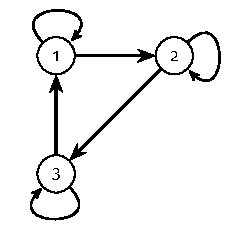
\includegraphics{./img/grafo_1.pdf}
\end{figure}

¿Está el grafo fuertemente conectado? Para $m=2$ sí, (puedo ir cualquier nodo a otro en 2 pasos, en el caso de los cortos por ejemplo sería: 1 a 2, 2 a 2)
\end{ejemplo}

\begin{ejemplo}
Determine la matriz de adyacencia del grafo:
\begin{figure}[H]
	\caption{Grafo dado.}
	\centering 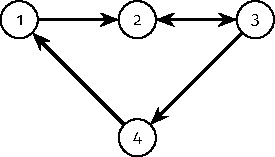
\includegraphics{./img/grafo_2.pdf}
\end{figure}

Solo tenemos que contar que la fila $i$-ésima son las flechas que llegan al nodo $í$-ésimo

$$ B =
\begin{pmatrix}
0 & 0 & 0 & 1 \\
1 & 0 & 1 & 0 \\
0 & 1 & 0 & 0 \\
0 & 0 & 1 & 0
\end{pmatrix}
$$

\begin{ejemplo}
Esta matriz es reducible (permutando la primera fila por la tercera), y además el grafo no está fuertemente conectado, lo que nos da una idea para la siguiente proposición.
\end{ejemplo}
\end{ejemplo}

\begin{nprop}
Sea $A\geq0$ de orden $dxd$, son equivalentes:
\begin{nlist}
\item $A$ es irreducible.
\item $graf(A)$ está fuertemente conectado.
\end{nlist}
\end{nprop}

\begin{nth}
Sea $A\geq0$ de orden $dxd$ e irreducible, entonces:
\begin{nlist}
\item $\lambda_{i}=\rho(A)$ es valor propio positivo y simple (no es dominante).
\item $\exists!u_{1}$ vector propio asociado a $\lambda_{1}=\rho(A)$ verificando $u_{1} >> 0$ y $\|u_{1}\|_{1}=1$, llamado vector de Perron.
\item Si $\exists j\in\{1,2,...,d\} : a_{ij} > 0 \implies \lambda_{i}=\rho(A)$ es dominante.
\item Todos los valores propios de módulo igual a $\rho(A)$ son simples.
\end{nlist}
\end{nth}

Sea $X_{n+1}=AX_{n},n\geq 0$, sistema lineal de ecuaciones en diferencias con solución: $X_{n}=A^{n}X_{0},n\geq 0$.
Si la matriz $A$ es positiva e irreducible vemos los casos posibles:
\begin{nlist}
\item $\lambda_{1}=\rho(A)$ es dominante, entonces:
\begin{nlist}
\item $\lim_{n\to\infty}X_{n}=0 \iff \rho(A) < 1$
\item Si $\rho(A)=1$ y $X_{0}\gg 0$, entonces $\lim_{n\to\infty}X_{n}=X >> 0$, que es vector propio asociado al valor propio $\lambda_{1}=1$
\end{nlist}
\item $\lambda_{1}=\rho(A)$ no es dominante, entonces habrá valores propios simples de igual módulo:
\begin{nlist}
\item $\rho(A)> 1$: las soluciones oscilan creciendo en radio.
\item $\rho(A)< 1$: las soluciones oscilan decreciendo hacia cero.
\item $\rho(A) = 1$: las soluciones se mantienen en la circunferencia unidad y podrían ser eventualmente periódicas.
\end{nlist}
\end{nlist}

\subsection{Matrices estocásticas. Cadenas de Markov}
\begin{ndef}[Matriz estocástica]
	Sea $A=(a_{ij})$ una matriz cuadrada de orden $d$ positiva. Se dice que $A$ es estocástica o de probabilidad o de Markov por columnas si
	$$\sum^{d}_{i=1}a_{ij}=1, \quad j=1,2,...,d$$
\end{ndef}

\begin{ejemplo}
Veamos si las siguientes matrices son de Markov:
\begin{nlist}
\item$I =
\begin{pmatrix}
1 & 0 & 0 \\
0 & 1 & 0 \\
0 & 0 & 1
\end{pmatrix}
$ es de Markov.
\item $A=
\begin{pmatrix}
0.5 & 1 & 0 \\
0.3 & 0 & 0.5 \\
0 & 0 & 0.5
\end{pmatrix}$ no es de Markov, falla para $j=1$
\item $B=
\begin{pmatrix}
0.3 & 0.1 & 0.7 \\
0 & 0.4 & 0.3 \\
0.7 & 0.5 & 0
\end{pmatrix}$ es de Markov.
\end{nlist}
\end{ejemplo}

\begin{nota}
\begin{nlist}
\item Las entradas de una matriz de Markov deben ser $0\leq b_{ij} \leq 1$
\item Las matrices de Markov pueden ser reducibles o irreducibles.
\end{nlist}
\end{nota}

\begin{nprop}
Sea A una matriz estocástica, entonces:
\begin{nlist}
\item $\rho(A)=1$ y además $\lambda_{1}=1$ es valor propio de $A$.
\item Admite un vector $v_{1}$ asociado a $\lambda_{1}=1$ con $v_{1}>0$.
\end{nlist}
\end{nprop}

\begin{proof}
Como $A$ es una matriz estocástica, debe ser positiva por tanto $A\geq 0$, luego podemos usar el criterio de las cotas por columnas (Proposición 4.4) que nos da $1 \leq \lambda_{1} \leq 1$ siendo $\lambda_{1}=1$ el mayor valor propio de $A$, luego queda demostrado.
\end{proof}

\begin{ndef}[Cadenas de Markov]
Una cadena de Markov es una sucesión de vectores positivos $\{P_{0},P_{1},...,P_{n},...\}$ solución de un sistema de ecuaciones en diferencias
$$ P_{n+1}=MP_{n}, \qquad n\geq 0,$$
donde $P_{0}$ cumple $\|P_{0}\|_{1}=1$, y se le llama distribución inicial de probabilidad, y la matriz de transición $M$ es estocástica.
\end{ndef}

\begin{nota}
Se tiene que con $\|P_{0}\|_{1}= 1 \implies \|P_{n}\|_{1}=1,n\geq 0$
\end{nota}

Las cadenas de Markov se utilizan para el estudio de repeticiones de experimentos con $d$ resultados posibles correspondientes a los estados $S_{1},S_{2},...,S_{d}$ con ciertas hipótesis:
\begin{nlist}
\item La probabilidad de que resulte un estado $S_{i}$ solo depende del resultado en la repetición anterior del experimento, y no de los anteriores.
\item $m_{ij},j=1,2,...,d$, representa la probabilidad de que se de el estado $S_{j}$ habiéndose dado el estado $j$ en la etapa anterior.
\item Sea $p_{n}(i)$ la probabilidad de que en la $n$-ésima repetición del experimento salga $S_{i}$. Entonces:
$$ p_{n+1}(i)=m_{i1}p_{n}(1)+m_{i2}p_{n}(2)+...+m_{id}p_{n}(d),$$
Por tanto:
$$\begin{pmatrix}
m_{11} & m_{12} & \cdots & m_{1d} \\
m_{21} & m_{22} & \cdots & m_{2d} \\
\vdots & \vdots & \vdots & \vdots \\
m_{d1} & m_{d2} & \cdots & m_{dd}
\end{pmatrix}
\begin{pmatrix}
p_{n}(1) \\
p_{n}(2) \\
\vdots \\
p_{n}(d)
\end{pmatrix}
=
\begin{pmatrix}
p_{n+1}(1) \\
p_{n+1}(2) \\
\vdots \\
p_{n+1}(d)
\end{pmatrix}
$$
Así, si $P_{n}=(p_{n}(1),p_{n}(2),...,p_{n}(d))^{t}$, entonces
$$P_{n+1}=MP_{n}, \qquad n\geq 0$$
Por el Teorema de la Probabilidad Total, si estoy en el estado $S_{j}$ solo puedo pasar a otro de los estados finitos $S_{1},...,S_{d}$ luego la suma de la columna $j$-ésima debe ser 1, que es lo mismo que decir que la matriz de transición $M$ es estocástica.
\end{nlist}

Hay dos tipos de cadenas de Markov:
\begin{nlist}
\item \underline{Cadenas regulares}: Una cadena de Markov es regular si la matriz $M$ es primitiva, es decir, $M^{k}>>0$ para algún entero positivo $k$. \\
En este caso, el valor propio $\lambda_{1}$ es dominante y por tanto la cadena que parte de un $P_{0}>>0$ tiende a una distribución estacionaria (vector propio asociado) de probabilidad que nos indican las probabilidades (proporciones) de cada uno de los estados del experimento a largo plazo.
\item \underline{Cadenas absorbentes}: Una cadena de Markov es absorbente si hay al menos un estado $S_{j}$ absorbente ($m_{ij}=1$) y desde cualquier otro estado podemos conectar a uno absorbente
\end{nlist}

\begin{ejemplo}
Un ejemplo de cadena absorbente sería el problema del borracho. En este problema nos imaginamos 4 puntos: un lago, una farola, un bar y la casa del borracho; de manera que están conectados en el orden que se han descrito (de la farola se puede ir al bar o al lago). El borracho sale del bar y tiene una probabilidad $p$ de girar a la derecha, y una probabilidad $q$ de girar a la izquierda, cumpliendo que $p+q=1$. Si el borracho llega a la casa, lo encierran (estado absorbente); si llega al lago se ahoga (estado absorbente).
\end{ejemplo}

\subsection{Aplicaciones}

\end{document}
